%
% this file is encoded in utf-8
% v2.0 (Apr. 5, 2009)

\documentclass[12pt, a4paper]{ntuthesis}

% 除非校方修改了論文格式 (margins, header, footer, 浮水印, 中文數字之章別)
% 或者需要增加所用的 LaTeX 套件,
% 或者要改預設中文字型、編碼
% 否則毋須修改本檔內容
% 論文撰寫,請修改以 my_  開頭檔名的各檔案

\usepackage{CJKutf8}  %%% ZZZ %%% macro for Chinese/Japanese/Korean processing
\usepackage{CJKnumb} %%% ZZZ %%% for Chinese numbering capability
\usepackage[nospace]{cite}  % for smart citation
%\usepackage{geometry}  % for easy margin settings
\usepackage{ntuthesis}
\usepackage{multirow,multicol,rotating}

%
% margins setting
%\geometry{verbose,a4paper,tmargin=3.5cm,bmargin=2cm,lmargin=4cm,rmargin=2cm}
%

% 插圖套件 graphicx
% 使用者工作流程是用 pdftex 還是 latex + dvipdfmx?
% 視情況而有不同的參數
% 這裡作自動判斷
% 參考自
% http://www.tex.ac.uk/cgi-bin/texfaq2html?label=ifpdf
\newcommand\mydvipdfmxflow{dvipdfmx}
\newcommand\mypdftexflow{pdftex}
\ifx\pdfoutput\undefined
  % not running pdftex
  \usepackage[dvipdfm]{graphicx}
  \newcommand\myworkflow{dvipdfmx}  % set the flag for hyperref
\else
  \ifx\pdfoutput\relax
    % not running pdftex
    \usepackage[dvipdfm]{graphicx}
    \newcommand\myworkflow{dvipdfmx}  % set the flag
  \else
    % running pdftex, with...
    \ifnum\pdfoutput>0
      % ... PDF output
      %\usepackage[pdftex]{graphicx}
      \newcommand\myworkflow{pdftex}  % set the flag
    \else
      %...DVI output
      \usepackage[dvipdfm]{graphicx}
      \newcommand\myworkflow{dvipdfmx}  % set the flag
    \fi
  \fi
\fi

% 增強功能型頁楣 / 頁腳套件
\usepackage{fancyhdr}  % 借用此套件來擺放浮水印 
% (佔用了 central header)
% 不需要浮水印的使用者仍可利用此套件,產生所需的 header, footer
%
% 啟動 fancy header/footer 套件
\pagestyle{fancy}
\fancyhead{}  % reset left, central, right header to empty
\fancyfoot[C]{\thepage} %中間 footer 擺放頁碼
\renewcommand{\headrulewidth}{0pt} % header 的直線; 0pt 則無線

% 如果不需要任何浮水印,則請把下列介於 >>> 與 <<< 之間
% 的文字行關掉 (行首加上百分號)
%% 浮水印 >>> 
%\input{yzu_watermark.tex}
%% <<< 浮水印

% 如需額外的頁楣 (header) 或 footer,請在 my_headerfooter.tex 裡依例修改
% 它的預設內容是都關掉,可依需要打開
%
% this file is encoded in utf-8
% v2.0 (Apr. 5, 2009)

%%%%%%% 其他的 header (left, right) 定義
% 底下定義了一些常見的 header 型式
% 預設情況是關掉的
% 使用者可以視需要將之打開
% 也就是把下列介於 >>> 與 <<< 之間
% 的文字行打開 (行首去掉百分號)

%% header >>>
%\renewcommand{\chaptermark}[1]{%
%\markboth{\prechaptername\ \thechapter\ \postchaptername%
%\ #1}{}%
%}  %定義 header 使用的「章」層級的戳記
%\fancyhead[L]{} % 左 header 為空
%\fancyhead[R]{\leftmark}  % 右 header 擺放「章」層級的戳記 (以 \leftmark 叫出)
%\renewcommand{\headrulewidth}{0.4pt}  % header 的直線 0.4pt; 0pt 則無線
%% <<< header

%%%%%%% 其他的 footer (left, right) 定義
% 底下定義了一些常見的 footer 型式
% 預設情況是關掉的
% 使用者可以視需要將之打開
% 也就是把下列介於 >>> 與 <<< 之間
% 的文字行打開 (行首去掉百分號)

%% footer >>>
%\fancyfoot[L]{} % 左 footer 為空
%\fancyfoot[R]{\small{YZU \LaTeX\ v2.0}} % 右 footer 擺放論文格式版本
%\renewcommand{\footrulewidth}{0.4 pt} % footer 的直線 0.4pt; 0pt 則無線
%% <<< footer




%%%%%%%%%%%%%%%%%%%%%%%%%%%%%%
%%%% 非必要的套件,但很實用
\usepackage{amsmath} % 各式 AMS 數學功能
\usepackage{amssymb} % 各式 AMS 數學符號
\usepackage{mathrsfs} %草寫體數學符號,在數學模式裡用 \mathscr{E} 得草寫 E
\usepackage{listings} % 程式列表套件
\usepackage{subfig}
\usepackage{tabularx}
\usepackage{url}
\usepackage[usenames,dvipsnames]{xcolor}
\usepackage{pgf}
\usepackage{tikz}
\usetikzlibrary{arrows,automata,positioning}



% Title Page
\renewcommand{\enTitle}{End-to-End Spoken Term Detection Based On Attention-based Nerual Network }  %英文標題
\renewcommand{\zhTitle}{基於專注式類神經網路之端對端口述詞彙偵測}  %中文標題
\renewcommand{\authorZhName}{敖家維}  %作者中文姓名
\renewcommand{\authorEnName}{Chia-Wei Ao}  %作者英文姓名
\renewcommand{\authorStudentID}{R04942094}  %作者學號
\renewcommand{\advisorZhName}{李宏毅}  %指導教授中文姓名
\renewcommand{\advisorEnName}{Hung-Yi Lee}  %指導教授英文姓名
\renewcommand{\zhCollegeName}{電機資訊學院}  %學院中文名稱
\renewcommand{\enCollegeName}{College of Electrical Engineering and Computer Science}  %學院英文名稱
\renewcommand{\zhDepartmentName}{電信工程學研究所}  %系所中文名稱
\renewcommand{\enDepartmentName}{Graduate Institute of Communication Engineering}  %系所英文名稱
\renewcommand{\rocYear}{一百零六}  %中華民國紀年年份
\renewcommand{\zhMonth}{七}  %中文月份
\renewcommand{\enYear}{2017}  %公元紀年
\renewcommand{\enMonth}{July}  %英文月份
\renewcommand{\oralDate}{106 年 7 月 10 日}  %口試日期

%
% listing setting
\lstset{breaklines=true,% 過長的程式行可斷行
extendedchars=false,% 中文處理不需要 extendedchars
texcl=true,% 中文註解需要有 TeX 處理過的 comment line, 所以設成 true
comment=[l]\%\%,% 以雙「百分號」做為程式中文註解的起頭標記,配合 MATLAB
basicstyle=\small,% 小號字體, 約 10 pt 大小
commentstyle=\upshape,% 預設是斜體字,會影響註解裏的英文,改用正體
%language=Octave % 會將一些 octave 指令以粗體顯示
}

\usepackage{url} % 在文稿中引用網址,可以用 \url{http://www.yzu.edu.tw} 方式

%%%% 以上為非必要套件
%%%%%%%%%%%%%%%%%%%%%%%%%%%%%%

%%% 以下是 hyperref 套件
%%%%%%%%%%%%%%%%%%%%%%%%%%%%%%
% hyperref 會擾亂 cite.sty 對文獻號碼縮編的排版,所以依據
% http://www.ctan.org/tex-archive/macros/latex/contrib/hyperref/
% 作如下的更動,使得 hyperref 不做文獻號碼的超連結。
\makeatletter
\def\NAT@parse{\typeout{This is a fake Natbib command to fool Hyperref.}}
\makeatother

% hyperlinkable table of contents
% 章節目錄、圖表超連結
\ifx\myworkflow\mydvipdfmxflow
	\usepackage[dvipdfmx, debug, colorlinks, linkcolor=black, citecolor=black, urlcolor=black, unicode]{hyperref}
\else
	\usepackage[pdftex, debug, colorlinks, linkcolor=black, citecolor=black, urlcolor=black, unicode]{hyperref}	
\fi

% if hyperref is not used (e.g., in LyX application)
% define dummy \phantomsection for those occurences
%   in yzu_frontpages.tex, yzu_backpages.tex, my_appendix.tex
\ifx\hypersetup\undefined
	\newcommand\phantomsection{}
\fi

% hyperref跟algorithm衝突,hyperref必須放在algorithm前面
\usepackage{algorithm}
\usepackage{algorithmic}
%%%% 以上為所有套件
%%%% 
%%%% 

% global page layout
%\newcommand{\mybaselinestretch}{1.5}  %行距 1.5 倍 + 20%, (約為 double space)
%\renewcommand{\baselinestretch}{\mybaselinestretch}  % 論文行距預設值
%\parskip=2ex  % 段落之間的間隔為兩個 x 的高度
%\parindent = 0Pt  % 段首內縮由 CJK 控制,所以這裡就設成不內縮

%%%%%%%%%%%%%%%%%%%%%%%%%%%%%
%  end of preamble
%%%%%%%%%%%%%%%%%%%%%%%%%%%%%
%
\begin{document}
\begin{CJK}{UTF8}{bsmi}   %%% ZZZ %%%  <<< 在這裡更改預設中文字型、編碼
% 編碼:UTF8, Bg5, ...
% 中文字型名稱:TeXLive 安裝有一套明體字 bsmi, 楷書與其他字型視你的 LaTeX CJK 系統裝設情況而定

% 針對 latex + dvipdfmx 工作流程在 hyperref 套件的影響下,圖檔的辨識力退化
% 所作的權宜措施。可能是因為 TeXLive2007 hyperref 裏的
% 客製 graphicx / dvipdfmx 的設定檔不夠新
\ifx\myworkflow\mydvipdfmxflow
	\DeclareGraphicsExtensions{.pdf,.png,.jpg,.eps}
	\DeclareGraphicsRule{.pdf}{eps}{.bb}{}
	\DeclareGraphicsRule{.png}{eps}{.bb}{}
	\DeclareGraphicsRule{.jpg}{eps}{.bb}{}
\fi

% global CJK setting
\CJKindent  %%% ZZZ %%%  段首內縮兩格

% 載入中文名詞的定義:例如,Figure -->「圖」, Chapter -->「第 x 章」
%
% this file is encoded in utf-8
% v2.0 (Apr. 5, 2009)

% 下列中文名詞的定義,如果以註解方式關閉取消,
% 則會以系統原先的預設值 (英文) 替代
% 名詞 \prechaptername 預設值為 Chapter
% 名詞 \postchaptername 預設值為空字串
% 名詞 \tablename 預設值為 Table
% 名詞 \figurename 預設值為 Figure
\renewcommand\prechaptername{第} % 出現在每一章的開頭的「第 x 章」
\renewcommand\postchaptername{章}
\renewcommand{\tablename}{表} % 在文章中 table caption 會以「表 x」表示
\renewcommand{\figurename}{圖} % 在文章中 figure caption 會以「圖 x」表示

% 下列中文名詞的定義,用於論文固定的各部分之命名 (出現於目錄與該頁標題)
\newcommand{\nameInnerCover}{書名頁}
\newcommand{\nameCommitteeForm}{論文口試委員審定書}
\newcommand{\nameCopyrightForm}{授權書}
\newcommand{\nameCabstract}{中文摘要}
\newcommand{\nameEabstract}{英文摘要}
\newcommand{\nameAckn}{誌謝}
\newcommand{\nameToc}{目錄}
\newcommand{\nameLot}{表目錄}
\newcommand{\nameTof}{圖目錄}
\newcommand{\nameSlist}{符號說明}
\newcommand{\nameRef}{參考文獻}
\newcommand{\nameVita}{自傳}



% 如果不需要以中文數字一、二、三呈現章別,例如「第一章」
% 則請把下列介於 >>> 與 <<< 之間
% 的文字行關掉 (行首加上百分號), 會以「第 1 章」呈現
%% 中文數字章別 >>>
%
% this file is encoded in utf-8
% v2.0 (Apr. 5, 2009)

% 請依需要選擇其中一種表現方式,把它所對應的指令列打開,其他沒有用到的表現方式的對應指令列請關閉。(用行首百分號)

%% 第一種目錄格式:
%%	1  簡介 ............................ 1
%%
%%      章別 (chapter counter) 「1」前後沒有其他文字,
%%
%%      內文章標題是
%%		第 1 章	簡介
%%	\tocprechaptername, \tocpostchaptername 都設成沒有內容的空字串
%%	\tocChNumberWidth 設成 1.4em (預設)
%%      底下三行指令請打開
%\renewcommand\tocprechaptername{}
%\renewcommand\tocpostchaptername{}
%\setlength{\tocChNumberWidth}{1.4em}


%% 第二種目錄格式:
%%	一、簡介 ............................ 1
%%
%%      章別 (chapter counter) 「一」前沒有文字,後有頓號,
%%
%%      內文章標題是
%%		第一章		簡介
%%	\tocprechaptername 設成沒有內容的空字串
%%	\tocpostchaptername 設成頓號
%%	\tocChNumberWidth 設成 2em
%%      底下四行指令請打開 (預設)
\renewcommand\countermapping[1]{\CJKnumber{#1}}
\renewcommand\tocprechaptername{}
\renewcommand\tocpostchaptername{、}
\setlength{\tocChNumberWidth}{2em}


%% 第三種目錄格式:
%%	第一章、簡介 ......................... 1
%%
%%      章別 (chapter counter) 「一」前有「第」,後有「章」與頓號,
%%      內文章標題是
%%		第一章		簡介
%%	\tocprechaptername 設成「第」
%%	\tocpostchaptername 設成「章、」
%%	\tocChNumberWidth 設成 3em
%%      底下四行指令請打開
%\renewcommand\countermapping[1]{\CJKnumber{#1}}
%\renewcommand\tocprechaptername{第}
%\renewcommand\tocpostchaptername{章、}
%\setlength{\tocChNumberWidth}{3em}



%% 可以依照需要作彈性的設定
%%
%% 章別 (數字,包括後面的字串) 的寬度 \tocChNumberWidth,
%% 會影響章名與章別之間的間隔 (太少則相疊,太多則留白)
%% 建議設成 \tocpostchaptername 內容字數加一,做為 em 的倍數,
%% 但至少也要有 1.4 倍。

%% <<< 中文數字章別

%%% 以下是載入前頁、本文、後頁
% 請勿更動
% 如需針對個別章節獨立編譯
% 請在 my_chapters.tex 檔裡對個別章節的 \input 指令以行首百分號方式做開關。

\NTUtitlepage  % 產生論文封面

\newpage
\setcounter{page}{1}
\pagenumbering{roman}

\NTUoralpage  % 產生口試委員會審定書

\mydoublespacing
\begin{acknowledgement} %誌謝
轉眼之間,碩士兩年就過去了。
\end{acknowledgement}

\begin{zhAbstract}  %中文摘要
本論文之主軸在探討語音數位內容之口述詞彙偵測。由於近年來網路蓬勃發展,使得網路上包含語音資訊的多媒體如線上課程、電影、戲劇、會議錄音等日漸增加,因此,語音數位內容之檢索也隨之受到重視。語音數位內容檢索的關鍵部分為口述語彙偵測,找出語音文件中出現查詢詞的部分。本論文
不經過語音辨識系統,使用機器學習中的類神經網路,在訓練語料中學習聲音的特徵,如此便可直接在語音訊號上進行口述詞彙偵測,以避免語音辨識系統錯誤率影響檢索系統的問題,也能夠避免經過語音辨識後,喪失掉許多語音中珍貴的資訊。

本論文將採用了專注式機制使模型能夠關注在語音文件的一部分,避免多餘的雜訊影響,以及回顧機制使模型依照之前的輸入關注在不同的地方。同時也使用了語音詞向量的概念,訓練出語音文件向量進行口述詞彙偵測。
\end{zhAbstract}

{
%\zhKaiFont
\mysinglespacing\selectfont
\tableofcontents %目錄

\listoffigures  %圖目錄

\listoftables  %表目錄
\par
}

\newpage
\setcounter{page}{1}
\pagenumbering{arabic}


\chapter{導論}
  \section{研究動機}
隨著網路跟電腦的普及,電腦資訊愈來愈豐富,使得我們尋找所需的資料變成一個大問題。因此,我們需要一套好的檢索系統
(Retrieval System)幫助我們快速地瀏覽資訊,並從中找到有用的部分,在過去已有許多文字檢索系統與演算法被開發出來並應用於產業中,如 Google Search、Microsoft Bing Search、Yahoo
Search等。隨著錄影音設備的普及,語音文件量正蓬勃地增加當中,隨著線上影片、會議錄音、線上課程等網站的興起,語音資料量越來越多,因此如何在其中找到使用者感興趣的資料便成為重要的議題,即為語音數位內容檢索(Spoken Content Retrieval)~\cite{chelba2008retrieval, lee2005spoken}。相較於文字資訊檢索,語音資訊檢索面臨到更多的挑戰,如辨識錯誤、辨識訓練資料不足等問題,使得此問題更形困難。

更由於行動裝置的出現,使用者可以不受地形時間限制,隨時取得資訊,促使許多網路公司一一推出了用語音輸入來檢索文字資訊的系統,如Google
公司推出的語音檢索功能即可讓使用者在手機或瀏覽器的介面上以語音輸入,由 Google 將其辨識成文字後再於 Google 的搜尋引擎上檢索資訊。 Apple 公司推出的個人語音助理 Siri,也讓使用者能以十分自然的方式對 Siri說出想要查詢的查詢詞(Query),由 Siri 辨識後在網路上檢索,並將檢索結果分門別類整理好後呈現給使用者看。如上述所說的這類檢索系統是用語音輸入的查詢詞去檢索大量的文字資訊,此方法稱為人聲檢索(Voice
Search),和本論文所探討的語音數位內容檢索(Spoken Content Retrieval)完全不同。

本論文所探討的語音數位內容檢索,是指由於網路上有大量的多媒體文件,如線上影片、會議錄音、線上課程、電視連續劇、演講等,而使用者也有搜尋這些多媒體文件的需求,此類允許使用者用文字或聲音輸入查詢詞並搜尋語音數位內容(Spoken Content)的系統稱為語音數位內容檢索,如 TED(美國著名的演講網站)會將網站上的演講內容轉寫(Transcript) 成為文字,並允許使用者於網站上輸入文字檢索這些影片的文字稿。 Youtube 也會於離線時將其網站上的影片辨識成文字,但目前尚不支援直接輸入查詢詞檢索影片轉寫的方式,可以期待未來 Youtube 會開放這方面的功能。只是上述兩個例子仍要倚賴人工的轉寫,要完全只靠機器自動辨識仍不容易做到。這種語音數位內容檢索將是本論文主要的研究主軸。

語音資訊檢索系統的效能取決於其前端語音辨識系統的效能,只要可以發展出完美的語音辨識系統,能夠完全正確的把聲音轉寫為文字,那需要將文件資訊檢索的方式套用到語音辨識的文字輸出上就解決語音資訊檢索這個問題了。依此邏輯來看,與其研究語音檢索,不如去研究如何提升語音辨識的正確率,而當完美的語音辨識系統被創造出來,語音檢索這個問題也就沒什麼好研究的了。因此TREC SDR track~\cite{trec}在2000年的時候即宣稱語音檢索在廣播新聞上(BroadcastNews)是一個「已解決的問題」(solved
problem),而在當時廣播新聞的辨識正確率已經到達90\%以上,但在自發性(Spontaneous)語音上,語音辨識正確率往往不到50\%,進而增加了在自發性語音上檢索的難度~\cite{saraclar2004lattice,mamou2006spoken},即使最近很流行的深度學習(Deep
Learning)大幅提升語音辨識系統的能力,語音辨識仍然是個困難的問題。短時間內語音辨識錯誤似乎是不可避免的,辨識錯誤對語音檢索所帶來的傷害幾乎在這個領域的每一篇論文的導論都會提到,用以彰顯語音檢索仍是個值得研究的問題,然而卻沒有太多方法能真正突破語音辨識錯誤所帶來的限制。並且傳統的語音數位內容之語意檢索系統主要的實作方法為先將語音文件辨識為文字檔後,對文字做檢索,但在辨識之中,會遇到如詞典外詞彙
(Out Of Vocabulary)、辨識錯誤等情況,更甚者,許多語音中珍貴的資訊如韻律(Prosody)、語速(Speaking Rate)和語者特徵(Speaker Characteristic)等在辨識後就消失了,十分地可惜。

本論文因此將語音辨識的部分移除,直接在語音訊號本身進行搜索,以類神經網路直接學習語音訊號的相似性,有別於傳統的聲學模型訓練強調辨識正確率的提升,本論文所提出的移除語音辨識,直接由語音訊號進行搜索提升語音檢索的效能。

\section{研究方向}
本論文之研究方向為使用類神經網路強化檢索系統之語音資訊檢索,主要包含以下幾點:

\begin{itemize}
\itemsep -2pt %reduce space between items
  \item
	  傳統的語意檢索系統是先將語音文件辨識為文字後,將輸入的文字查詢詞進行檢索,語音辨識系統的影響會直接反應在搜尋結果上,但自動語音辨識系統(Automatically Speech Recognition)
的訓練是很昂貴的,需要大量標注完善的語料才能訓練出很好的聲學與語言模型。因此,利用類神經網路擁有有良好的推廣性(Generization)
和適應性(Adaptability)強的優點,直接對於語音信號本身搜索,避免語音辨識的錯誤。
  \item
	  更進一步地,由於語音文件無法跟文字文件一樣清楚分段,對於模型來說計算量是很龐大,且充斥著雜訊。因而,引進了專注式機制(Attention
	  Mechanism),來使模型能夠將目光注目特定的位置上,減少雜訊的干擾,進而學習出更好的向量表示(Vector Representation)
  \item
	  由於學習的向量表示,會過度貼近(Overfit)訓練資料,導致推廣性的下降。使用自動編碼器(Auto-encoder)\cite{vincent2008extracting,li2015hierarchical,baldi2012autoencoders}
	  產生文字向量(Word2vec),語音向量(Audio2vec)\cite{mikolov2013distributed,mikolov2013efficient,pennington2014glove,chung2016audio},進而進行搜索。
  \item   再者,利用了成對學習法 (Pairwise
	  Learning)使得原本的分類問題加入了排序(Ranking)的概念,使得系統能夠更加精準的分出正確資料與錯誤資料間的差異,進而提升檢索系統。
  \item
	  最後,將上述的模型統整在一起,將語音向量當作正規化(Regularization),利用畫重點機制排除多餘雜訊,提升模型的效能,使搜尋結果更加進步。

\end{itemize}

\section{章節安排}
本論文之章節安排如下:

\begin{itemize}
\itemsep -2pt %reduce space between items
  \item  第二章:介紹本論文相關背景知識。
  \item  第三章:介紹如何以類神經網路實現口述詞彙偵測。
  \item  第四章:介紹如何以畫重點機制類神經網路實現口述詞彙偵測。
  \item  第五章:介紹如何產生語音向量跟文字向量,並應用於口述詞彙偵測
  \item  第六章:介紹如何以成對學習法訓練檢索系統。 
  \item  第七章:介紹將畫重點機制跟語音向量同時應用在口語詞彙偵測。
  \item  第八章:本論文之結論與未來研究方向。
\end{itemize}


\chapter{背景知識}
  \section{資訊檢索與語音資訊檢索}

\subsection{資訊檢索}


資訊檢索 (Information Retrieval,IR)
是指從資料庫中擷取出與某個主題(Topic)相關之檢索對象(Object)的行為。基本使用流程為:使用者輸入了一段查詢對象 $ Q $ (Query),系統能夠從資料庫中傳回和這個主題相關的檢索對象(Object),並進一步依據檢索對象和主題的相關程度進行排序(Ranking),以方便使用者瀏覽並取得所需的檢索對象。如圖\ref{fig:ch2_IR}。
\begin{figure}
\centering
\includegraphics[scale=0.4]{images/ch2_Ir.png}
\caption{資訊檢索系統基本架構} \label{fig:ch2_IR}
\end{figure}

檢索對象  $ x $ 
指的是系統所檢索出的東西,例如:在文字搜尋中檢索對象指的是文章、在網路檢索中指的是網頁、在圖像檢索指的是圖片、在語音檢索指的是口語片段(Spoken Segment)等,同時,查詞對象  $ Q $  也可以為圖片、文字或聲音。
本篇論文中所使用的查詢詞  $ Q $  形式有二:文字構成的字串、口述形式。本篇論文使用  $ x $  則都是語音文件。

當有了查詢對象,系統的主要任務就是去計算相關性(Relevance),其定義為  $ P(R|x,Q) $  ,然後依此機率大小對檢索對象進行排序,這個排序方式
被稱為機率排序原則 (Probability Ranking Principle,PRP)\cite{robertson1997probability}。
這個相關性函式通常是按照檢索系統的需求去決定的,可以是用機器學習(Machine
learning)的方法學習出來,也可以是由系統設計者決定。上述的方法可以視為一個分類問題(Classfication),另一種方法為排序學習(Learning
to Rank),此時系統不在需要計算  $ P(R|x,Q) $ ,而是尋找一個排序函式(Ranking Function)
 $ S(x,Q) $ ,能夠將 $  S(x_T,Q)>s(x_F,Q) $ ,  $ x_T $  為相關的檢索對象、  $ x_F $ 
為不相關的檢索對象。也就是說,所有相關的檢索對象,都能夠超過不相關的檢索對象。

如何檢驗一個資訊系統的好壞也是重要的課題首先我們必須要準備測試集,其中包含文件資料庫、查詢詞、以及與每個查詢詞對應的相關文件的標註。藉由評估系統在測試集上於「正確度」、「速度」、以及「佔用空間」等數個面向的表現,以了解此系統與其他系統的優劣比較。

文字檢索會議 (The Text REtrieval Conference,TREC),自1992年起每年的居舉行會議,並在多個測試項目上提供大規模之標準測試集,藉此讓來自世界各地的參加團隊評估自己的系統效益同時與其他團隊相互討論切磋。如今,TREC除英文的檢索測試集外,更提供了非英文的大規模檢索測試集
(如西班牙文與中文)、語音檢索測試集、以及跨語言檢索測試集。另外在測試項目上也有了多樣的發展,包括引入了開放領域自動問答
(Open-Domain Question Answering)以及基於內容的數位影音檢索
(Content-based Retrieval of Digital Video)
等。資訊檢索已是一門受到關注的領域。



\subsection{語音資訊檢索}
目前語音檢索可以分為兩類,「口述語彙偵測 (Spoken Term
Detection)」與「語意檢索 (Semantic
Retrieval)」,本論文著重在口述詞彙偵測,在此將兩者簡介如下:

\subsubsection{口述語彙偵測}


口述語彙偵測的目的是檢索出所有包含查詢詞的語音文件,著重於逐詞比對(Literal
Term
Matching),主要有兩種檢索情境。第一種是先將語音文件辨識為詞圖(Lattice)後,當使用者輸入文字的查詢詞後,系統會在詞圖上進行查詢詞的檢索。這種檢索情境需要有訓練好的自動語音辨識系統(Automatic Speech Recognition,ASR),由於語音辨識系統並無法保證在所有情況下都有很好的辨識率,因此由辨識錯誤所導致的檢索性能下降是在此最需要解決的問題。過去的文獻有用聲學特徵如梅爾倒頻譜係數
(Mel-Frequency Cepstral Coefficients (MFCC))幫助分類器 (Classifier)
在分類一篇語音文件是否相關時的判斷,也有利用相關回饋 (Relevance Feedback)、圖論 (Graph)與隨機漫步 (Random Walk)
解決這些問題。

第二種是非監督式
(Unsupervised),的方法,查詢詞與語音文件都是語音形式的,也有人稱之為依例查詢
(Query-by-Example),系統直接利用如動態時間校準(Dynamic Time Warping)
等方法在信號上比對語音文件中是否有某一段聲音與查詢詞很相像,過去的方法通常是為了解決不同文件間語速上的差異提出如有斜率限制的動態時間校準(Slope-Constraint
DTW),或是為了解決動態時間校準逐一比對所有文件庫所花時間過多的問題。計算此情境下的
 $ S(Q, x) $  為利用片段式動態時間規劃 (Segmental Dynamic Time Warping),簡介於~\ref{sec:chap4_sdtw}。

\subsubsection{語意檢索}
語意檢索的目的為回傳概念上相關的語音文件,而不一定要出現查詢詞。希望查詢結果與輸入的查詢詞是概念上匹配(Concept
Matching)的,而不是只回傳有出現查詢詞的文件,如當使用者查詢「美國總統」,文件中包含「美國總統」、「美國白宮」,而不是與查詢詞完全一樣的文件,通常也是使用者想要的。文字領域的資訊檢索已經有「概念匹配」的做法來達到語意檢索,但是由於文字領域的資訊檢索是在文字為完全正確的狀況下,不像語音數位文件的檢索往往會有辨識錯誤的問題。對於語音文件,一個較常見的實作方法通常是使用相關回饋(Relevance Feedback)~\cite{ruthven2003survey} 與查詢詞擴展(Query Expansion)~\cite{voorhees1994query,xu1996query}。

\subsection{片段式動態時間校準 (Segmental DTW)}
\label{sec:chap4_sdtw}
口述語彙偵測的目的為搜尋整個語料庫後,找出其中有出現查詢詞的語音文件,同時找出這些語音文件中可能有出現查詢詞的假設區域 (Hypothesized Region) ,並給這個假設區域一個相關分數,最後系統再根據相關分數進行排序後回傳給使用者 (分數較高為較相關)。

這裡考慮的口述語彙偵測是查詢詞也是語音形式的情境。此時所用的方法為片段式動態時間校準 (Segmental Dynamic Time Warping)~\cite{chan2010unsupervised, hazen2009query}。假設輸入的查詢詞的特徵為 $ \mathbf{X} = (\mathbf{x}_1, ..., \mathbf{x}_{|\mathbf{X}|}) $ ,語音文件的特徵為 $ \mathbf{Y} = (\mathbf{y}_1, ..., \mathbf{y}_{|\mathbf{Y}|}) $ ,有了這兩者之後,就可以建立一個距離表格 (Distance Table)  $ D(i, j) = \rho(\mathbf{x}_i, \mathbf{y}_j) $ ,通常這裡使用的特徵是
高斯事後機率 (Gaussian Posteriorgrams)~\cite{zhang2009unsupervised}或是梅爾倒頻譜係數
(MFCC)。如果使用高斯事後機率的話,兩個音框之間的距離為
 $ \rho(\mathbf{x}_i, \mathbf{y}_j) \equiv -\log (\mathbf{x}_i
\cdot\mathbf{y}_j) $ 。如果使用梅爾倒頻譜係數的話,兩個音框之間的距離為兩點之間的歐幾里得距離(Euclidean
Distance),即 $ \rho(\mathbf{x}_i, \mathbf{y}_j)
\equiv\sqrt{|\mathbf{x}_i - \mathbf{y}_j|^2} $ 。

動態時間校準的目的是要在  $ D(i, j) $  上找一條距離總合最短的路徑從  $ (1, s) $  到  $ (|\mathbf{X}|, e) $  表示從  $ \mathbf{X} $ 對應到 $ (\mathbf{y}_s, ..., \mathbf{y}_e) $  (因為查詢詞一定要被完全對應,而語音文件不一定要被完全對應到)。由於假設區域可以出現在語音文件中的任何地方, 因此片段式動態時間校準將距離表格  $ D(i, j) $  切成數個重疊的對角片段 (寬度為  $ R $ ),所以說每個片段的起始點分別為  $ (1, 1), (1, 1+R), (1, 1+2R),... $  如圖 ~\ref{fig:chap4_sdtw} 所示,每個對角片段都代表了一個可能出現查詢詞的區域,所以要在每個對角片段上找出距離總合最短的路徑,即這個對角片段上的假設區域。片段式動態時間校準會從每個片段中找出一段距離總合最短的路徑,在每個片段中所有對應的路徑 (Warping Path) 都必須要完整地待在片段內,不可超出片段。

\begin{figure}[h]
\centering
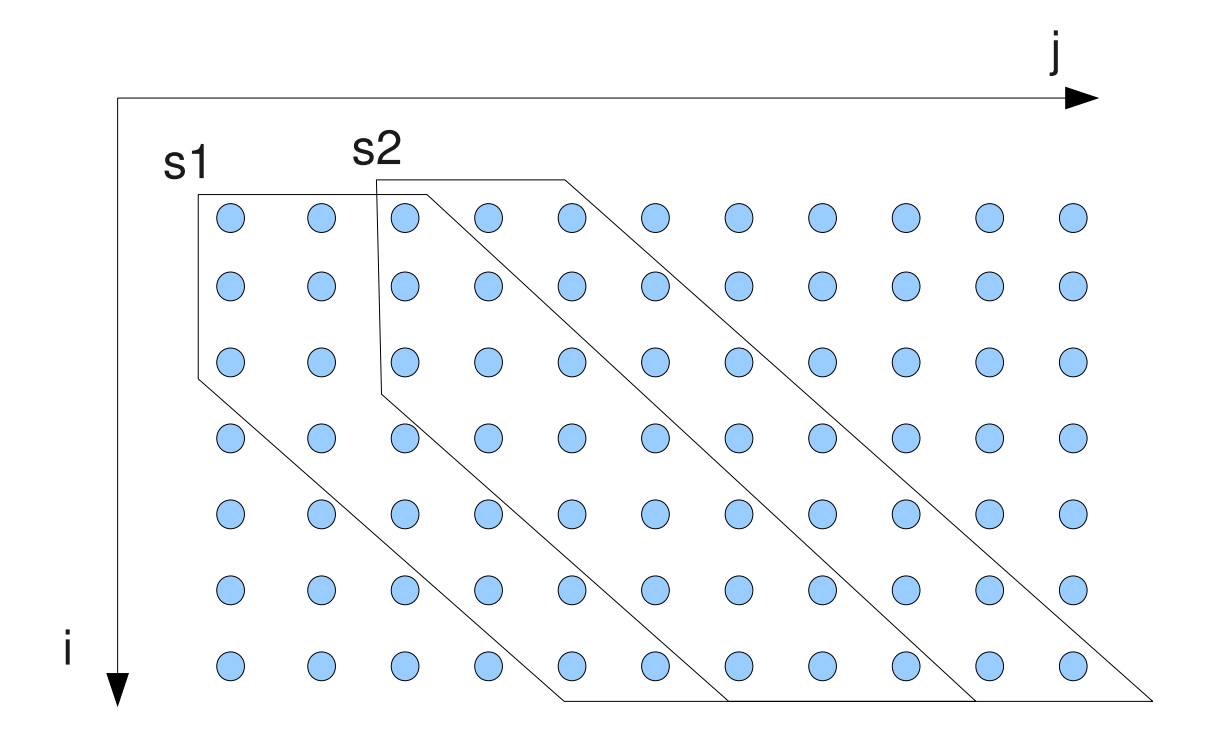
\includegraphics[scale=0.3]{images/chap4_sdtw.png}
\caption{片段式動態時間校準示意圖~\cite{zhang2009unsupervised}} \label{fig:chap4_sdtw}
\end{figure}

假設在每個片段中的對應路徑為:

\[
\phi = (i_t, j_t), t = 1,...,|\phi|
\]

代表著如下的對應關係:

\[
\mathbf{x}_{i_1} \leftrightarrow \mathbf{y}_{j_1}, \mathbf{x}_{i_2} \leftrightarrow \mathbf{y}_{j_2},...,\mathbf{x}_{|\phi|} \leftrightarrow \mathbf{y}_{|\phi|},
\]
而邊界條件是  $ i_1 = 1, i_{|\phi|} = |\mathbf{X}| $  , $ j_1 $  為  $ 1+kR $  ,對應路徑中所有的點都要在片段內,即:

\[
|(i_t-i_1)-(j_t-j_1)| <= R
\]

而片段式動態時間校準的目標是要在每個片段內找到一條路徑  $ \phi $  使得下式的距離總和最小:

\begin{equation}
C_{\phi}(\mathbf{X}, \mathbf{Y}) = \sum_{t=1}^{|\phi|} \rho(\mathbf{x}_{i_t},\mathbf{y}_{j_t})
\end{equation}

\begin{figure}[h]
\centering
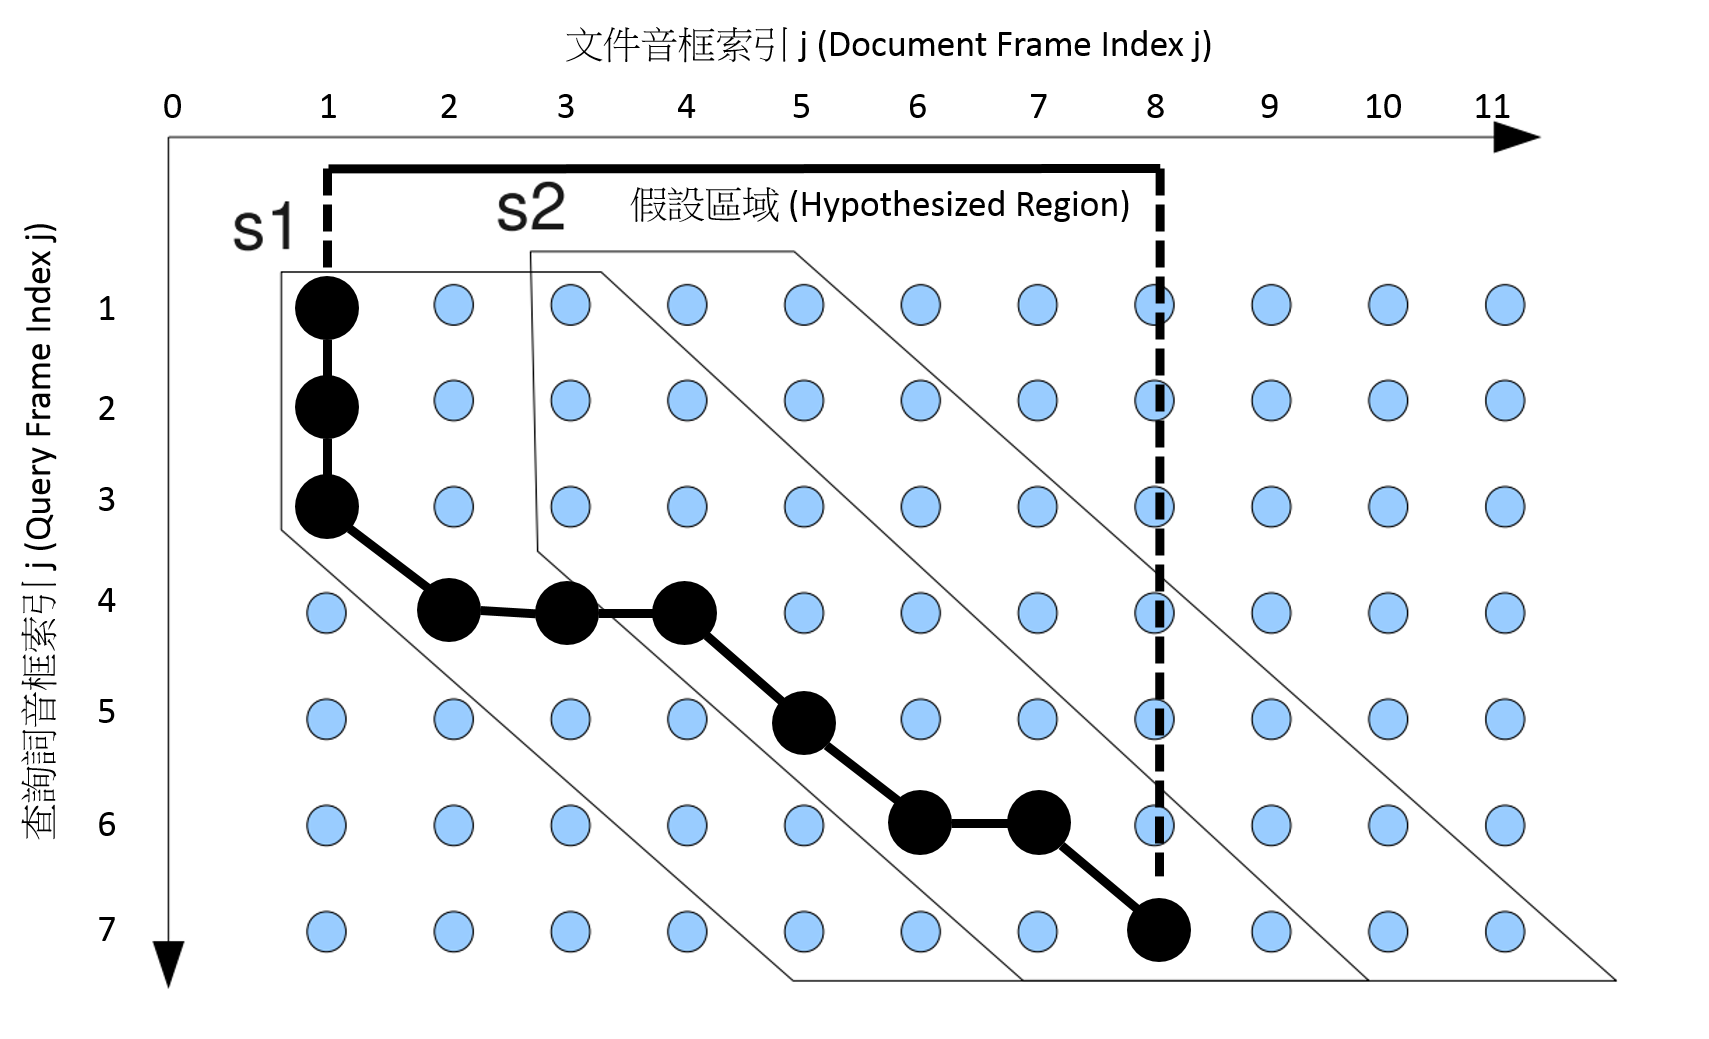
\includegraphics[scale=0.4]{images/chap2_segdtw_exp1.png}
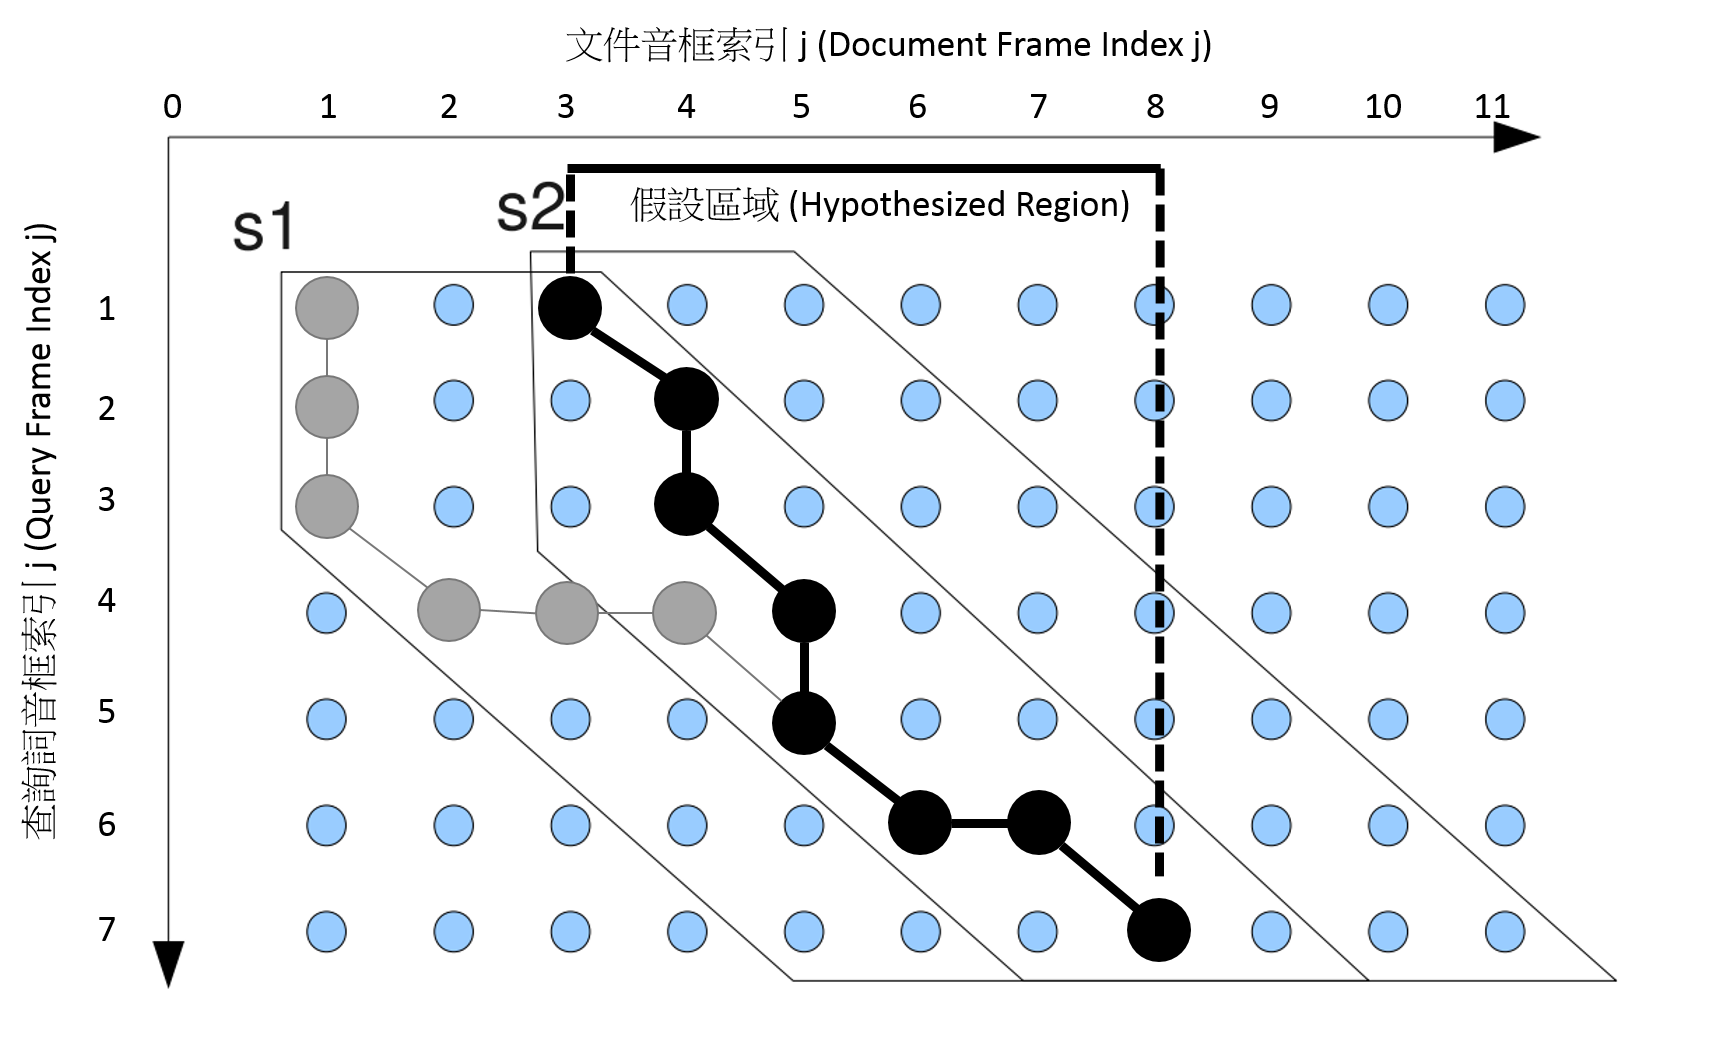
\includegraphics[scale=0.4]{images/chap2_segdtw_exp2.png}
\caption{示意如何從兩個對角片段中找到相關分數最大的假設區域,其中  $ R=2 $ }
\label{fig:chap2_sdtw_exp}
\end{figure}




每個片段中使得  $ C_{\phi}(\mathbf{X}, \mathbf{Y}) $  最小,即使得相關分數  $ -C_{\phi}(\mathbf{X}, \mathbf{Y}) $  最大的那條  $ \phi $  即為每個片段中的假設區域  $ (\mathbf{y}_{j_1},...,\mathbf{y}_{j_{|\phi|}}) $  ,而在每個片段中找到最大相關分數的路徑可以使用動態規劃 (Dynamic Programming) 求解。圖~\ref{fig:chap2_sdtw_exp}中顯示了兩個對角片段與其對應的最大相關分數的路徑與假設區域。圖中上半部中的  $ (\mathbf{y}_1, ..., \mathbf{y}_8) $  代表在第一個對角片段中找到的假設區間,圖中下半部中的  $ (\mathbf{y}_3, ..., \mathbf{y}_8) $  則是在第二個對角片段中找到的假設區域。 找到所有假設區域後,將假設區域按照其與查詢詞的相關分數進行排序後,即為口述語彙偵測的結果。在一篇語音文件中找到所有可能的假設區域需要  $ O(|\mathbf{X}||\mathbf{Y}|) $  的計算量來計算點與點之間的距離  $ \rho $ ,並需要 $ O(|\mathbf{X}||\mathbf{Y}|) $ 的計算量來找到相關分數最大的路徑。

\vspace{20mm}
\subsection{資訊檢索評估機制}
為了有效比較彼此系統,制訊檢索評估機制的標準是很重要的一環,本節將對一些常見以及本論文所使用的評分標準一一做介紹。

\subsubsection{準確率(Precision)與召回率(Recall)}
檢索系統找出的所有可能相關檢索對象中,真正相關的比例稱之為準確率,準確率高代表所找出的檢索結果的可信度高;
而所有真正的相關檢索對象有多少比例被系統檢索出來,我們稱之為召回率,召回率高代表系統找回越多相關的檢索目標。通常會為系統設定一個閥值(Threshold),文件的分數若高於閥值,則視為相關,反之若文件的分數低於閥值,則視為不相關。準確率和召回率的定義如下:

\[
\text{準確率}=\frac{\text{檢索到的相關檢索對象數}}{\text{檢索到的檢索對象數}}
\]

\[
\text{召回率}=\frac{\text{檢索到的相關檢索對象數}}{\text{所有的相關檢索對象數}}
\]

通常這兩個值彼此之間的關係為負相關。調高閥值的話準確率會上升,但召回率則會下降;反之若調低閥值,準確率會因此下降,召回率則會很高。可以考慮一個極端例子:當閥值非常低時,幾乎所有的文件都是相關文件,此時的召回率相當於1,但準確率就會很低了。因此單看準確率或召回率是無法準確地評估系統的優劣的,必須要兩者一起評估。

\begin{figure}
\centering
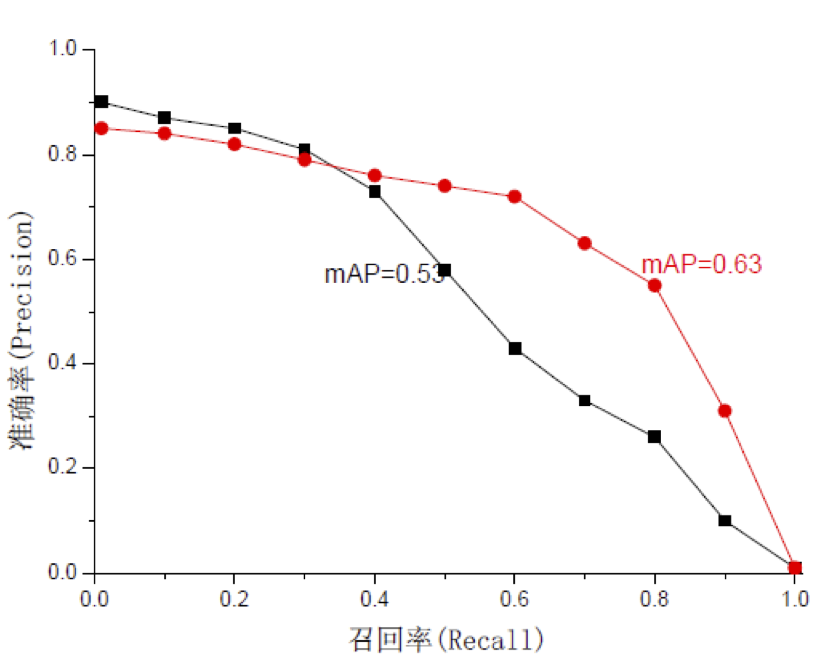
\includegraphics[scale=0.5]{images/chap2_precision_recall.png}
\caption{準確率、召回率和平均準確率之關係} \label{fig:precision_recall}
\end{figure}

\subsubsection{P@N}

通常使用者最重視的是檢索系統傳回的前幾名結果,所以就發展出了 $ P@N $ 這個評估機制。 $ P@N $ 就是只看前N個檢索結果的正確率。例如:前五個檢索結果中有一個是相關的,那 $ P@5 $ 就是20\%。

 $ P@N $ 的定義如下:
\[
P@N=\frac{\text{前N個文件裡的相關文件數}}{N}
\]
 然而由於不同的查詢詞其相關的檢索對象數不同,因此  $ P@N $  有時候並非公平的評比方式, 舉
 例來說,如果整個資料庫裡面相關的檢索對象只有5個,  $ P@10 $  最高就只能到
 0.5。
\subsubsection{平均準確率~\cite{garofolo2000trec}}

因為準確率和 $ P@N $ 都需要事先決定,當查詢詞和條件不同時,很難準確地評估兩個系統的效能。因此有人提出了平均準確率(Mean Average Precision, MAP)的概念,如圖~\ref{fig:precision_recall},平均準確率就是準確率和召回率曲線下面積的平均值。平均準確率的定義如下:
\begin{equation}
MAP = \frac{1}{|Q|} \sum_Q \frac{\sum_{d \in D^R}precision(d)}{|D^R|}
\end{equation}
其中Q代表查詢詞的集合, $ |Q| $ 為查詢詞的總數, $ D^R $ 為和查詢詞Q相關的文件d的集合, $ |D^R| $ 代表和查詢詞Q相關的文件數量。precision(d)代表系統檢索出文件d時的準確率。




\section{深層類神經網路(Deep Neural Network, DNN)}
\label{DNN}
\subsection{簡介}
深層類神經網路發想於生物的神經系統結構。神經系統由非常多的神經元組成,彼此以樹突、軸突與突觸連結,每顆神經元自己有活化閾值來決定激發
態與否。根據此仿生的觀察,便產生一種數學模型(如圖~\ref{fig:ch2_bio_neuron}與~\ref{fig:ch2_math_neuron}),將其層層疊起(如圖~\ref{fig:ch2_DNN}),即為深度類神經網路的全貌。
\begin{figure}[hb]
\centering
\subfloat[][生物學上的單顆神經元結構]{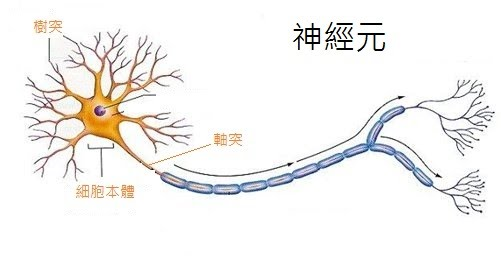
\includegraphics[scale=0.3]{images/ch2_bio_neuron.jpg}\label{fig:ch2_bio_neuron}}
\subfloat[][數學上的單顆神經元結構(感知器)]{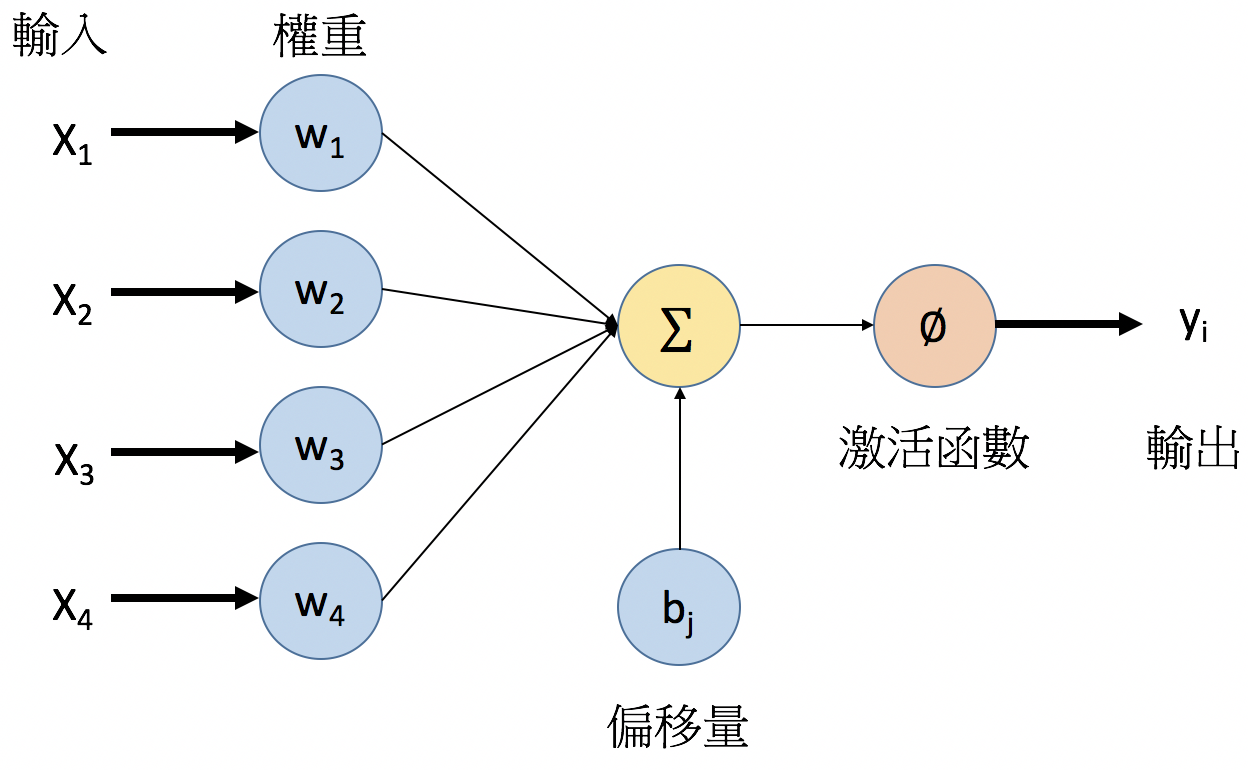
\includegraphics[scale=0.3]{images/ch2_single_neuron.png}\label{fig:ch2_math_neuron}}
\caption{類神經網路的單顆神經元}
\end{figure}

\begin{figure}[h]
\centering
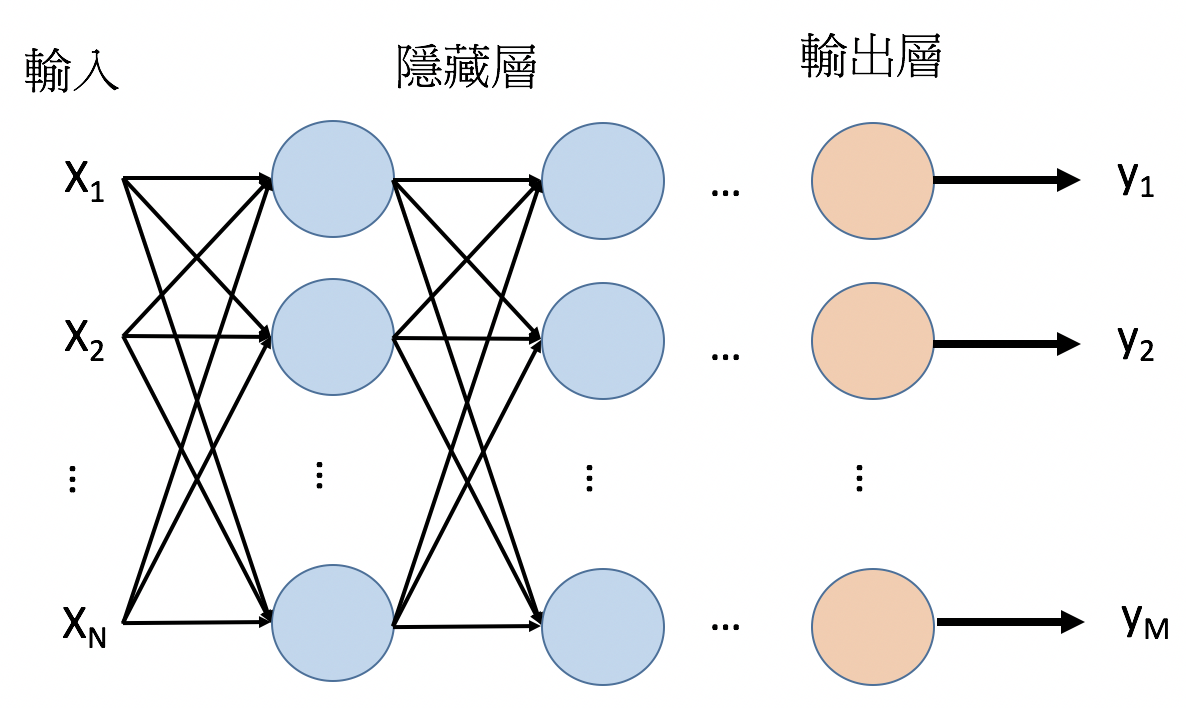
\includegraphics[scale=0.3]{images/ch2_DNN.png}
\caption{基本深度類神經網路架構圖} \label{fig:ch2_DNN}
\end{figure}

深度類神經網路是目前機器學習重要的一個分支,曾經在1980年代蓬勃發展,但因計算代價太高,且同時有其他簡單的模型如支撐向量機(Support
Vector Machine)的興起而沒落。深層學習的概念由辛氏(Geoffrey Hinton)於2006重新推出~\cite{hinton2006fast},並使用一種新型的訓練方法,能夠有效提升訓練的執行速度;加上圖形處理器(Graphics
Processing
Unit,GPU)大幅提高了數值和矩陣運算的速度,使得深層類神經網路重新成為機器學習領域中的重要角色。
\subsection{運作原理}
類神經網路的架構如圖~\ref{fig:ch2_DNN},其結構由感知器(Perceptron)~圖\ref{fig:ch2_math_neuron}串接而成,因此深層類神經網路又稱為多層感知器(Multi-layer
Perceptron,MLP)。每一層根據所在位置可分為三類:
\begin{itemize}
\item    輸入層(Input Layer): 即為類神經網路輸入特徵向量(Feature Vector) $ \bold{X} = [x_1 , x_2 , x_3 , x_4 ... , x_N]^T $ 
\item    隱藏層(Hidden Layer): 類神經網路的主要部分,可以有很多層,且每層的感知器(神經元)數目可以不同。
\item    輸出層(Output Layer): 跟隱藏層很相似,不過會依據模型的目的有所改變。譬如回歸問題,此時輸出層就不會經過活化函數。對於分類問題,輸出層的數量會跟標記種類(Class)相同。
\end{itemize}

每個感知器都包含了一組加權係數跟偏移量(Bias),跟非線性的活化函數(Activation
Function)。數學式如下:
\begin{equation}
	y_i = \phi{(\sum_{i=1}^{M} w_{ij}x_i+b_j) }
\end{equation}

其中 $ \phi $ 是活化函數, $ w_{ij} $ 是第 $ j $ 個感知器中,對應到第 $ i $ 個輸入 $ x_i $ 的加權係數, $ b_j $ 是第 $ j $ 個感知器的偏移量。 $ \phi $ 括號內的特徵轉換稱為仿射變換(Affine
Transformation)。可將之想像為一個從 $ M $ 維實數空間映射到 $ N $ 維實數空間的函數 $ A:
R^M \rightarrow R^N $ ,其中 $ M $ 和 $ N $ 分別是輸入向量 $ x $ 與輸出向量 $ y $ 的維度。由於仿
射變換可看成是一個線性矩陣的轉換,複雜度並不夠高,因此我們引入 $ \phi $ 這個非線性的活化函數。常見的活化函數分別為S型函數(Sigmoid)和整流線性單元(Rectified Linear Unit, ReLU)。
\begin{equation}
\begin{aligned}
&sigmoid(x) = \frac{1}{1 + e^{-x}}
\\
&ReLU(x) = max( 0 , x )
\end{aligned}
\end{equation}


\subsection{訓練類神經網路}
\label{ch2_train_DNN}
深層類神經網路常見的訓練方法為反向傳播演算法(Back
Propagation)\cite{rumelhart1988learning},通常要搭配一些最佳化演算法(Optimization
Method)例如梯度下降法(Gradient Descent)。
其概念為模型會計算出當下錯誤的程度,並依照可以減少錯誤的方向更改參數。為了定義錯誤的程度,需借用到損失函數(Loss
Function)來定義錯誤,其訓練的目標可以規劃為以下的最佳化問題(Optimization
Problem):
\begin{equation}
\min_{\theta}{ \sum_{n=1}^{N}{ {L( \bold{x}_n , \bold{y}_n ,\theta)}}}
\end{equation}
損失函數通常是要能夠反應在你預想的輸出跟模型的輸出的真實距離。損失函數的值越大,代表模型的輸出結果與期望目標相差越遠,也因此訓練的目標為最小化損失函數,所以定義一個好的損失函數是很重要的。

以多類別分類器為例,分類器的輸出 $ \hat{\bold{y}} $ ,會將每一個維度對應到一個分類標籤,共有 $ C $ 種類別。屬於正確標籤的 $ \bold{y} $ 表示為一個獨一餘零(1-hot)的向量 $ [0, 0 , ... , 0 , 1 , 0 ... , 0]^T  $ ,只有正確類別  $ l $  的值是1,其餘為0。訓練此種分類器時,損失函數常為交叉熵(Cross Entropy, CE),定義為:
\begin{equation} 
\label{eq:LCE}
L_{CE}(\bold{x} , \bold{y} , \theta) = KL( \bold{y} || f_{\theta}(\bold{x}) ) = KL(\bold{y} || \hat{\bold{y} }) = \sum_{i = 1}^{C} y_i \log{ \frac{y_i}{\hat{y}_i} } = - \log \hat{y}_{l} 
\end{equation}
其中 $ KL(p||q) $ 代表的是克雷散度(Kullback–Leibler Divergence),用以衡量兩組機率分佈的距離,值越大則代表兩組分佈越不相似。 $ L_{CE}(\bold{x} , \bold{y} , \theta)  $ 計算了分類器的正確標籤 $ \bold{y} $ 與通過模型參數後的預測向量 $ \hat{\bold{y}} $ 的克雷散度,但由於 $ C $ 種正確標籤中,只有一個類別 $ l $ 的值為1,也因此 $ L_{CE}(\bold{x} , \bold{y} , \theta)  $ 可以簡化成公式\ref{eq:LCE}最右邊的簡單型態,最小化正確分類標籤的負對數可能性(Negative Log Likelihood, NLL)。

以多類別回歸器而言,則更廣義地希望將回歸器的輸出向量 $ \hat{\bold{y}} $ 與目標向量 $ \bold{y} $ 的距離拉近。訓練此種分類器時,距離的衡量通常為均方差(Mean Square Error, MSE),定義為:
\begin{equation}
L_{MSE}(\bold{x} , \bold{y} , \theta) = || \bold{y} - f_{\theta}(\bold{x}) ||_2 = || \bold{y} - \hat{\bold{y}} ||_2 = \sum_{i = 1}^{C} ( y_i - \hat{y}_i )^2 
\end{equation}

當設計者決定好損失函數後,下一步是選擇解決最佳化問題的演算法。理想上,理想參數應能夠最小化損失函數:
\begin{equation}
\theta^* = \arg\min_{\theta}{ \sum_{n=1}^{N}{ {L( \bold{x}_n , \bold{y}_n , \theta)}}}
\end{equation}

但因類神經網路中間含有非線性活化函數的緣故,最小化損失函數通常沒有解析解(Analytical
Solution),或稱封閉解(Close-form Solution)。實務面上,通常採用迭代式(Iterative)演算法,給定一個參數起點,一步一步減少損失函數。
最簡單的迭代式最佳化演算法為統計式梯度降低(Stochastic Gradient Descent, SGD)演算法,給定某一組參數 $ \theta $ ,損失函數沿著該參數上的梯度方向更新,下降的速度最快,可表達成:
\begin{equation}
	\begin{aligned}
	&\theta_{k+1} \leftarrow \theta_k - \eta \Delta \theta_{k} 
	\\
	&\Delta \theta_{k} = \frac{\partial L}{\partial \theta} \biggr|_{\theta = \theta_k}
	\end{aligned}
\end{equation}
其中 $ \eta $ 為學習率(Learning rate),調控最佳化的速度與精細度, $ k $ 為更新的迭代次數,隨著 $ k $ 的增加,可期望損失函數的值越來越小,模型越接近理想模型。


在使用SGD訓練深度類神經網路的時候,通常是使用反向傳播(Back
Propagation)演算法,在模型完成順向預測(Forward
Prediction)計算出 $ \hat{\bold{y}} $ 後,會先得到最後一層參數的梯度值,再根據鏈鎖律(Chain-rule),將梯度反向傳播回輸入層,取得每一層的參數的梯度值,從而完成更新。


\subsection{類神經網路的困難}
\begin{itemize}
\item{局部最佳解(Local Optimum)}

	使用最佳化演算法訓練類神經網路的時候,沒有任何方法可以保證損失函數是下凹(Convex)的。在損失函數下降的過程中,並不保證會下降到最佳解(Global Optimum) 上,很有可能會停在局部最佳解上。因此在訓練之初通常使用隨機初始化,並且擴增模型的隨機性,以避免掉落到結果較差的局部最佳解上。

同時梯度的計算牽扯到函數的一次微分,對於雜訊的反應較不穩健,訓練上不穩定。更進階的訓練方式包含了慣量(Momentum),使得每次SGD更新的時候,包含了前次更新的梯度方向,可表達為:
\begin{equation}
\Delta \theta_{k} =  \mu \Delta \theta_{k-1} + \frac{\partial L}{\partial \theta} \biggr|_{\theta = \theta_k}
\end{equation}
其中 $ \mu $ 為慣量係數,用以調控慣量的比例,來降低卡在局部最佳解上的機率。
\item{ 過度貼合(Overfitting)}
	
	機器學習常會遇到過度貼合(Overfitting)的問題,亦即模型在訓練資料表現越來越好,但在測試資料中損失函數越變越差。模型為了在訓練資料中表現好,而是將所有訓練資料背誦,無法學習到真正幫助分類與回歸的本質,導致因此模型的推廣性(Generization)下降。常見的避免過度貼和的方法為正規化(Regularization)跟丟棄演算法(Dropout)~\cite{srivastava2014dropout}。

	1. 正規化的目的在於減弱模型的複雜度,也就是對於模型參數大小做限制,即是是在原本的損失函數中,加入 $ ||\theta||_p $ 如\ref{eq:L2}:
\begin{equation}
\label{eq:L2}
\begin{aligned}
&\min_{\theta}{ \sum_{n=1}^{N}{ {L( \bold{x}_n ,\bold{y}_n,\theta)}}+\lambda||\theta||_p^p}
\\
&||\theta||_p = ( \sum_{\theta_i \in \bold{\theta}}{|\theta_i|^p} )^\frac{1}{p}
\end{aligned}
\end{equation}
其中 $ ||\theta||_p $  稱為  $ L^p $  範數 (  $ L^ p $   norm) , λ 則是一個介於 0 到 1 之間的係數。
當  $ p = 1 $  時,稱為一次正規化(L1 Regularization)。而  $ p =
2 $ 時,為二次正規化(L2 Regularization)
。一次正規化使模型 $ \bold{\theta} $ 
中傾向出現較多的 $ 0 $ ,故常稱為稀疏解(sparse solution)。二次正規化對於模型
 $ \bold{\theta} $ 
絕對值較大的參數給予較多的懲罰,避免其中的 $ \bold{\theta_i} $ 值太大或太小,來減少模型的複雜度來避免避免過度貼合現象。由於類神經網路中, $ \bold{\theta} $ 
多半是層與層之間的權重矩陣 $ \bold{W} $  ,故二次正規化也常被稱為權重衰減 (weight
decay)。

2. 丟棄演算法(dropout),在每次訓練中,模型內每個神經元會有 $ p $ 的機率直接被丟棄,使得輸出值為0,如圖\ref{fig:ch2_drop1}和\ref{fig:ch2_drop2}。藉由隨機丟棄,可以讓模型中的各種參數自力更生,使模型學到更概括化的能力。

\begin{figure}[ht]
\centering
\subfloat[][未經丟棄的DNN]{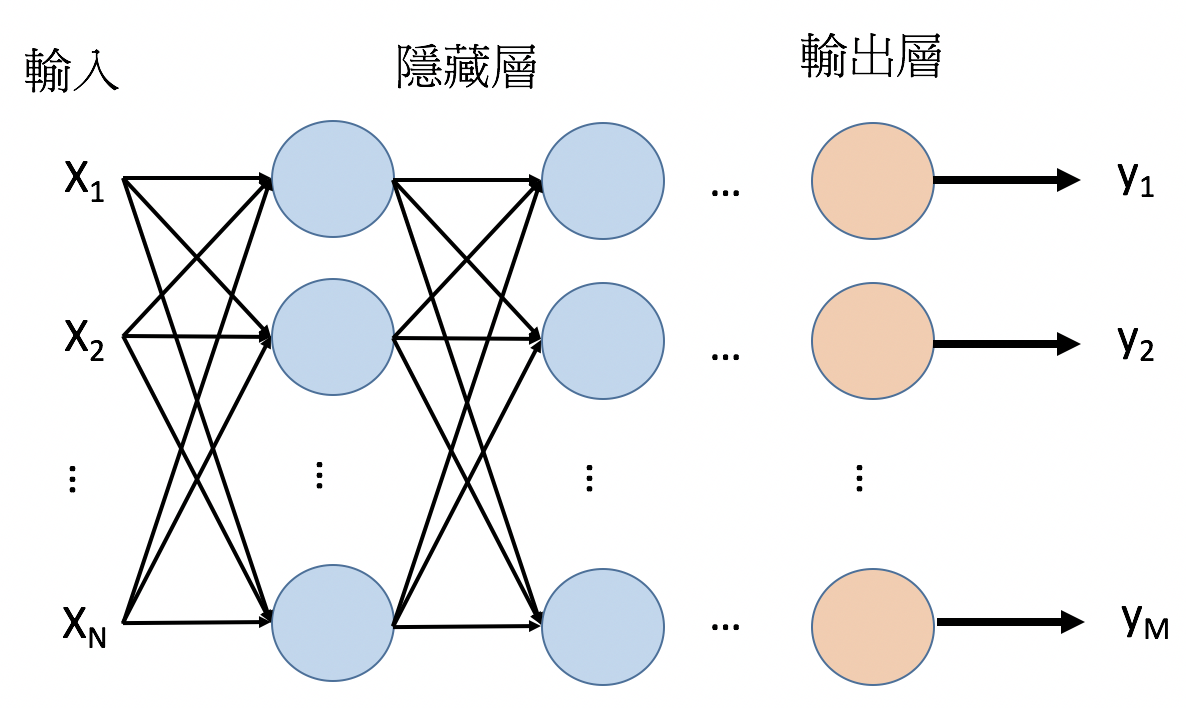
\includegraphics[scale=0.25]{images/ch2_DNN.png}\label{fig:ch2_DNN_no_drop}}
\subfloat[][隨機丟棄的DNN]{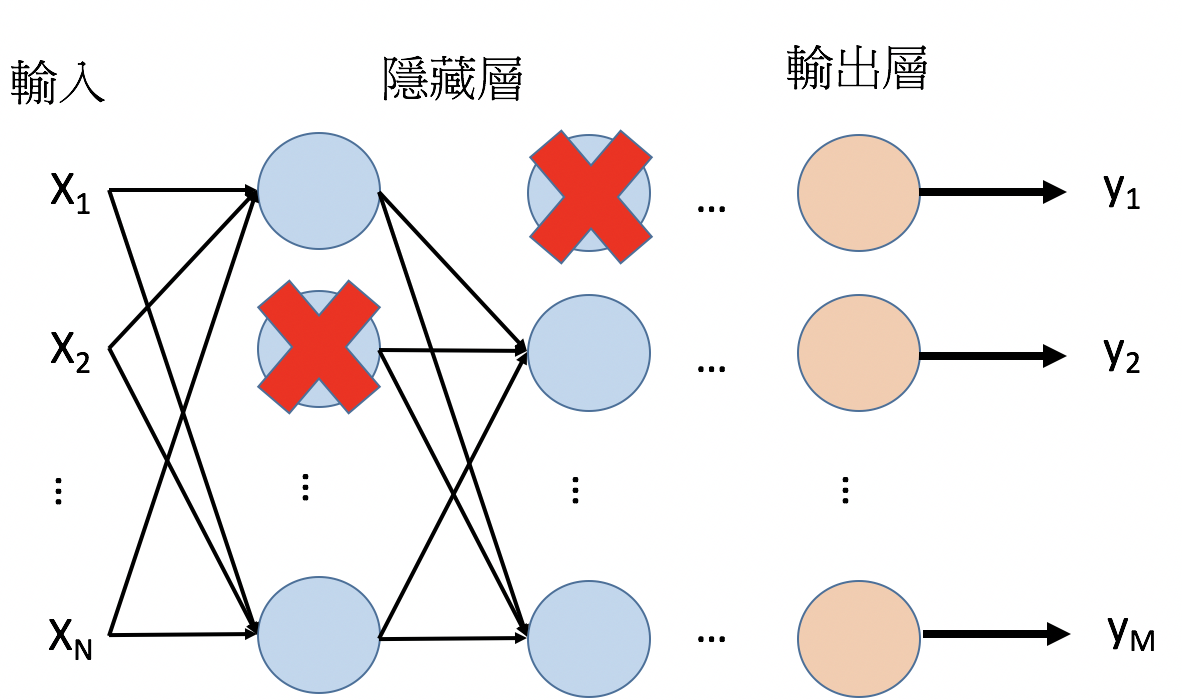
\includegraphics[scale=0.25]{images/ch2_dropout1.png}\label{fig:ch2_drop1}}
\subfloat[][隨機丟棄的DNN]{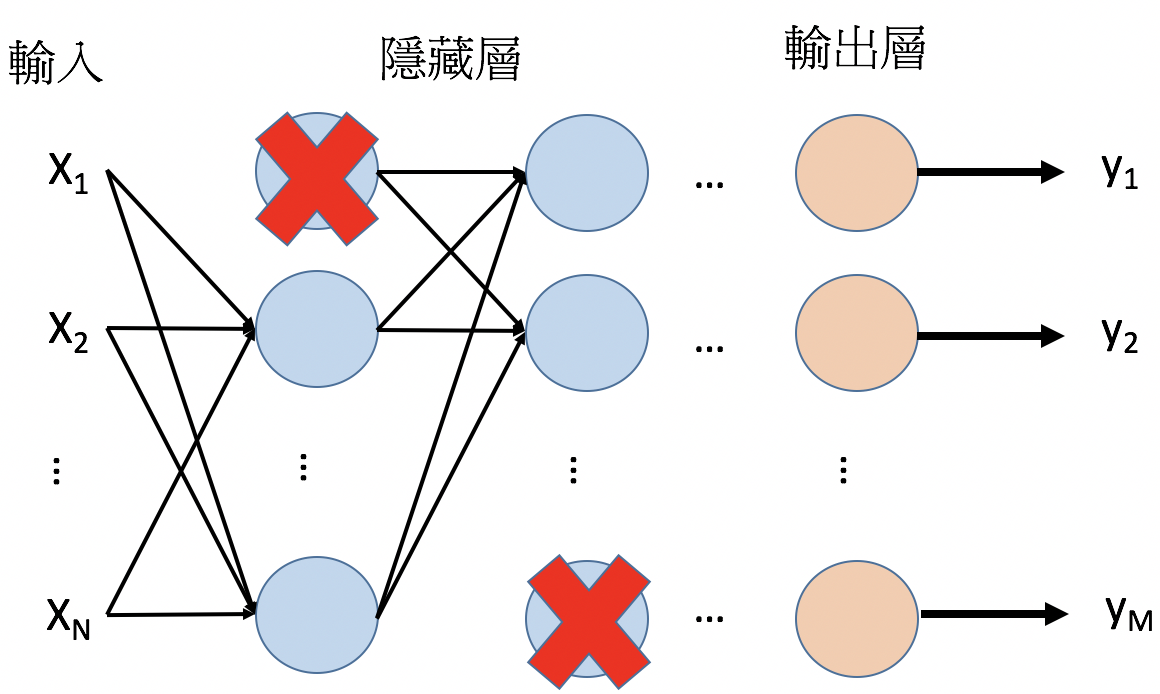
\includegraphics[scale=0.25]{images/ch2_dropout2.png}\label{fig:ch2_drop2}}
\caption{丟棄演算法}
\end{figure}
	丟棄演算法同時也可以視為隨機整合(Random Ensemble)模型。整合模型
	(Ensemble Model)在機器學習領域已經被證明是非常強大的模型,藉由多個模型的多樣性(Diversity)各司其職,提昇模型強度。類比在丟棄演算法中,根據不同的丟棄情況,有不同的神經元組合互相整合而成。隨機性造就了多樣性,又同時控制調適,使得模型更不容易過度貼合。

\end{itemize}
\section{遞迴式類神經網路(Recurrent Neural Network,RNN)}
\subsection{簡介}
類神經網絡已經是非常強大的模型,但對它而言,每次輸入都是獨立的,它並不記得曾經有過什麼樣的
輸入。這樣的類神經網絡對於有時序性(Sequential),且有上下文關係(Context
Dependency)的輸入時,例如語音辨識(Speech
Recognition)和自然語言理解(Naturl
Language Understanding),便無法表現得太好。因此讓類神經網路加上記憶的能力,即為遞迴式類神經網路(Recurrent
Neural Network)~\cite{elman1990finding}。

\begin{figure}[h]
\centering
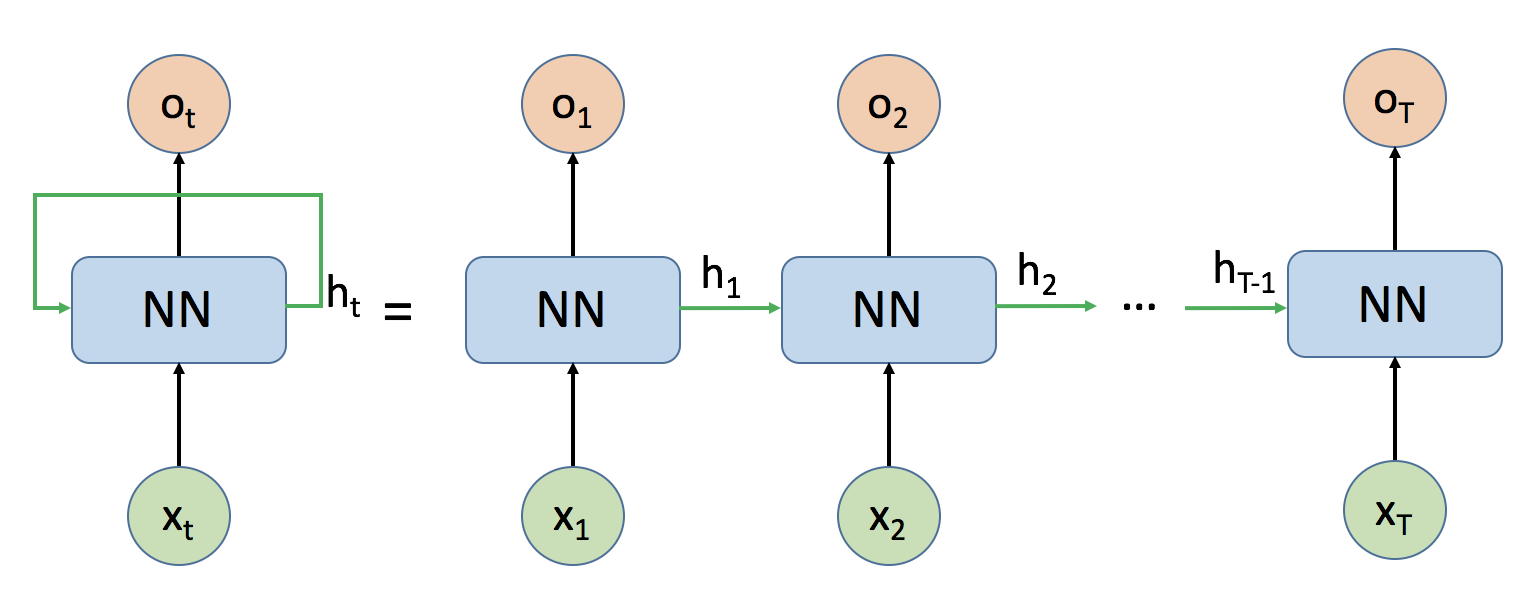
\includegraphics[scale=0.5]{images/ch2_RNN.png}
\caption{遞迴式類神經網路架構圖} \label{fig:ch2_RNN}
\end{figure}
\subsection{運作原理}
	圖~\ref{fig:ch2_RNN}為模型架構, $ NN $ 為一組類神經網路, $ x_t,o_t,h_t $ 為時間點t的輸入、輸出跟記憶。透過記憶細胞,類神經網路能夠將之前輸入的資訊往後傳遞,並且影響後面的輸出。如下式\ref{eq:h_t}。
\begin{equation}
\label{eq:h_t}
\begin{aligned}
&h_t = \phi_h{(W_h x_t+U_h h_{t-1}+b_h)}
\\
&o_t = \phi_o{(W_o h_t+b_o)}
\end{aligned}
\end{equation}
記憶 $ h_t $ 會跟時間  $ t $  的輸入  $ x_t $  與上個時間點的記憶  $ h_{t-1} $  影響。
其中 $ W_h,W_o,U_h,b_o,b_h $ 為遞迴式類神經網路的參數, $ \phi_h,\phi_o $ 為活化函數。



\subsection{沿時間反向傳播演算法}
沿時間反向傳播演算法 (back propagation through time)~\cite{werbos1990backpropagation}的概念跟反向傳播演算法類似,其唯一不同的是每個時間的梯度(Gradient)會沿著時間往前傳,如圖\ref{fig:ch2_BPTT}紅色的梯度和綠色的梯度都會一直往前傳,更新模型的參數。實務上,須根據所設定的展開時間層數,往前傳播,且訓練後個時間點的隱藏層與隱藏層間的權重矩陣將取平均,以讓個時間點的權重相同。
\begin{figure}[ht]
\centering
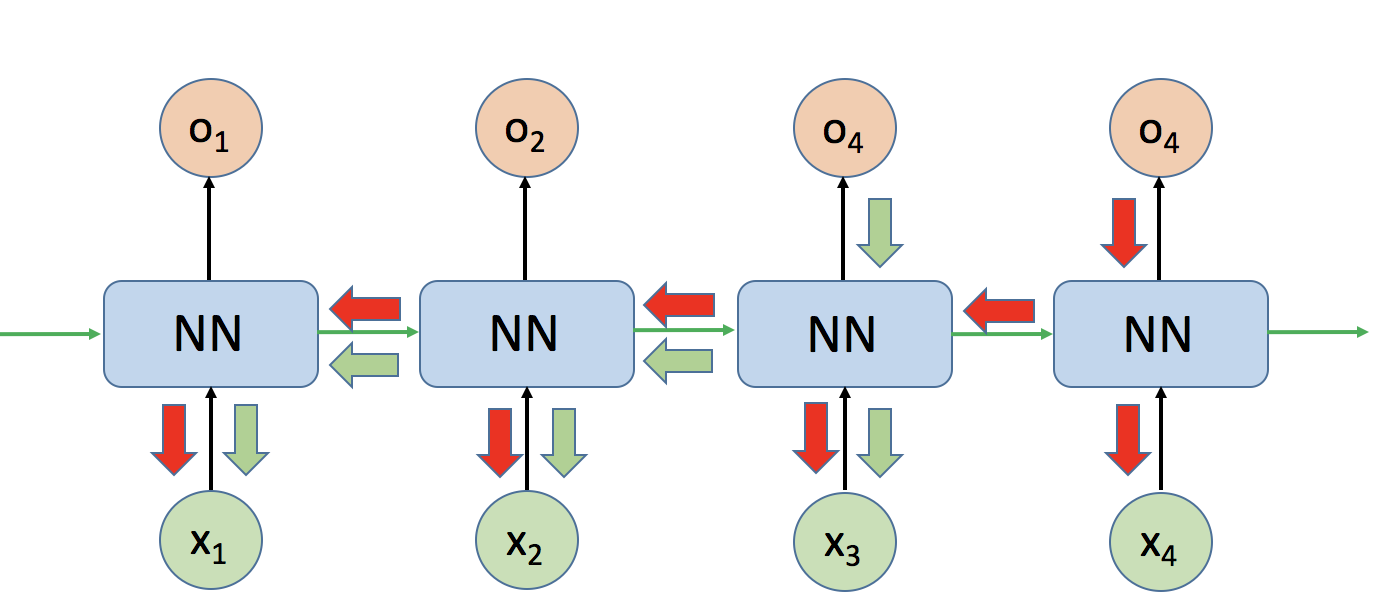
\includegraphics[scale=0.5]{images/ch2_BPTT.png}
\caption{沿時間反向傳播演算法的示意圖} \label{fig:ch2_BPTT}
\end{figure}

\subsection{長短期記憶神經網路}
\label{LSTM}
隨著輸入序列的長度加長,遞迴神經網路無法記得一開始的資訊,同時跟人類一樣,我們不需要記憶每個時間點的資訊,只需要記憶關鍵的資訊。因此更近一步提出一種進階形式:長短期記憶網路(Long Short-term Memory
Network)\cite{gers2001long},是一種特殊的遞迴神經網路,能夠彌補之前的缺點。
長短期記憶網路,比一般遞迴神經網路來得複雜,將原本的類神經元由長短期記憶細胞(Long
Short-term Memory Cell)取代,如圖\ref{fig:ch2_lstm},在每個時間點,這組神經網路會有一個單元狀態(Cell
State),並使用三個被稱作門限(Gate)的機制來輔助管理、移除、以及新增資訊。以下將會詳細說明各門限及其運作方式。
\begin{figure}[ht]
\centering
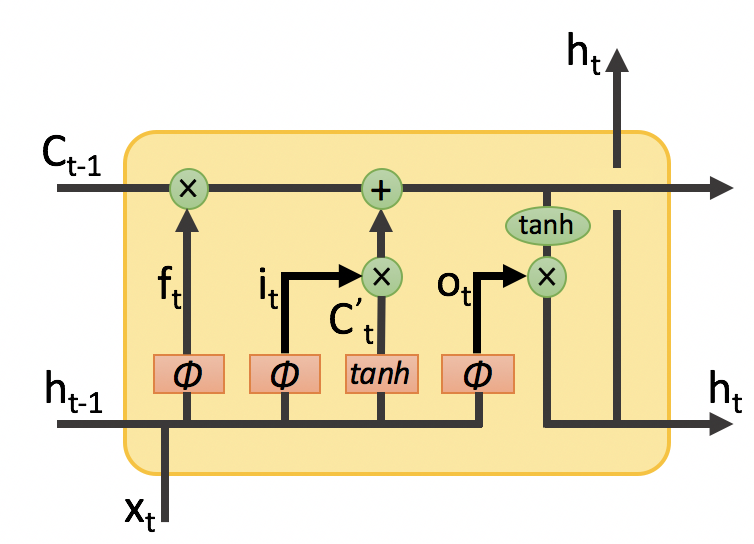
\includegraphics[scale=0.5]{images/ch2_lstm.png}
\caption{長短期記憶細胞的示意圖\cite{shen2016}} \label{fig:ch2_lstm}
\end{figure}
\begin{itemize}
\item{遺忘門限(Forget Gate) $ f_t $ }
	
	負責決定哪些資訊需要從單元狀態中丟棄。
	如式子\ref{eq:forget_gate}跟圖\ref{fig:ch2_forget_gate},依照前一個時序的輸出以及現在的輸入,產生一個值介於 $ 0 $ 到 $ 1 $ 的向量,藉由跟前一單元狀態 $ C_{t-1} $ 進行逐點乘積(Pointwise
	Product)時,可以決定哪些值要被捨棄多少。其中 $ \phi $ 表S型函數、 $ x_t $ 為第 $ t $ 個時刻的輸入、 $ h_{t-1} $ 則為前一時刻的輸出。
\begin{equation}
\label{eq:forget_gate}
f_t =  \phi( W_{xf} x_t + W_{hf} h_{t-1}+b_f)
\end{equation}
\begin{figure}[ht]
\centering
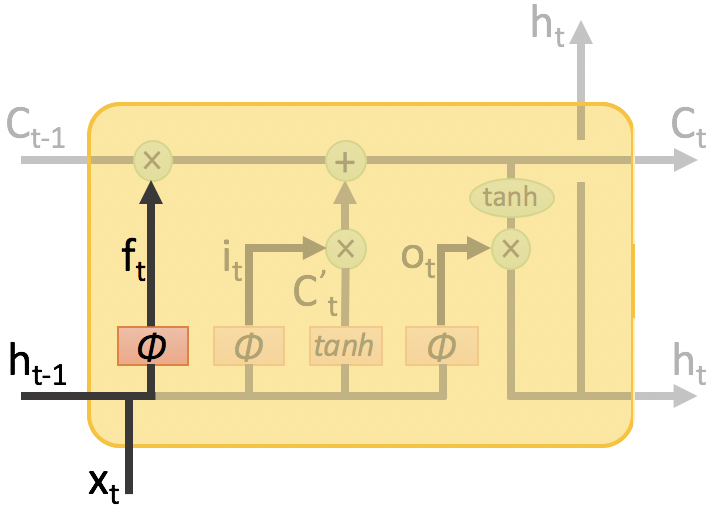
\includegraphics[scale=0.5]{images/ch2_forget_gate.png}
\caption{遺忘門限的運作圖\cite{shen2016}} \label{fig:ch2_forget_gate}
\end{figure}
\item{輸入門限(Input Gate) $ i_t $ } 

負責控制輸入訊息,假如模型認為是此時輸入為雜訊,可以將輸入門限設為0,反之設為1。另一個非線性函數雙曲正切(Hyperbolic
Tangent,tanh)將負責產生此時間點儲存資訊的候選值 $ C'_t $ 。如式\ref{eq:input_gate},圖\ref{fig:ch2_input_gate}所示。
\begin{equation}
\label{eq:input_gate}
\begin{aligned}
&i_t = \phi( W_{xi} x_t +W_{hi} h_{t-1} +b_i)
\\
&C'_i = tanh( W_{xC} x_t +W_{hC} h_{t-1} +b_C)
\end{aligned}
\end{equation}
\begin{figure}[ht]
\centering
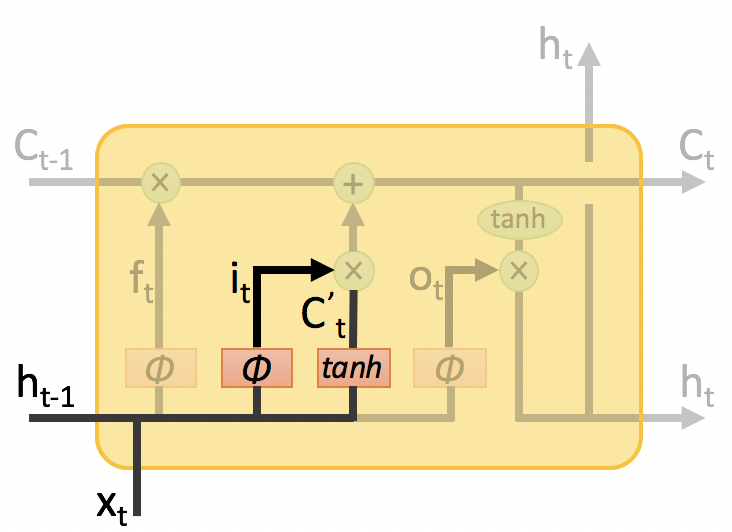
\includegraphics[scale=0.5]{images/ch2_input_gate.png}
\caption{輸入門限的運作圖\cite{shen2016}} \label{fig:ch2_input_gate}
\end{figure}
\item{更新單元狀態(Cell State)}

基於上面幾個運算,現在可以更新單元狀態,如式\ref{eq:update},圖\ref{fig:ch2_update}。新的單元狀態為上一個時間點的單元狀態 $ C_{t-1} $ 乘上遺忘門限 $ f_t $ 與此時的單元狀態候選 $ C'_t $ 乘上輸入門限 $ i_t $ 相加。
\begin{equation}
\label{eq:update}
C_t = f_t * C_{t-1} + i_t * C'_t
\end{equation}
\begin{figure}[ht]
\centering
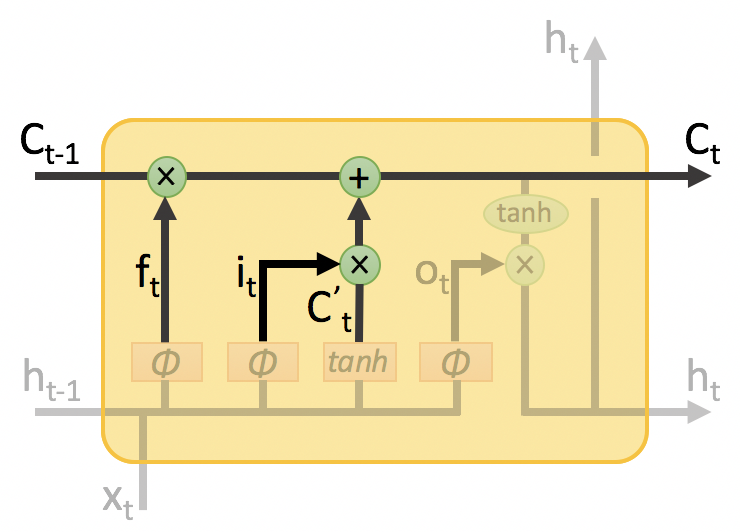
\includegraphics[scale=0.5]{images/ch2_update.png}
\caption{更新單元狀態的運作圖\cite{shen2016}} \label{fig:ch2_update}
\end{figure}
\item{輸出門限(Output Gate) $ o_t $ }

輸出門限 $ o_t $ 控制模型的輸出結果,其運作方式為與將通過雙曲正切函數的單元狀態 $ C_t $ 產生出 $ h_t $ ,進行逐點乘積,如此使模型能夠輸出想要的部分。如式\ref{eq:output_gate},圖\ref{fig:ch2_output_gate}所示。
\begin{equation}
\label{eq:output_gate}
	\begin{aligned}
		&o_t = \phi (W_{xo} x_t +W_{ho} h_{t-1} +b_o)
		\\
		&h_t = o_t * tanh(C_t)
	\end{aligned}
\end{equation}
\begin{figure}[ht]
\centering
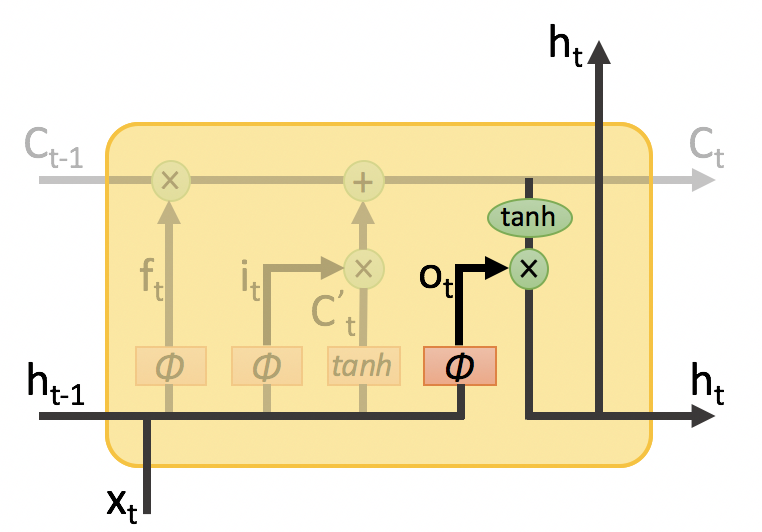
\includegraphics[scale=0.5]{images/ch2_output_gate.png}
\caption{輸出門限的運作圖\cite{shen2016}} \label{fig:ch2_output_gate}
\end{figure}
\end{itemize}

因上述的門限控制,可以使新的類神經網路,控制自己想要記憶的東西,而不是每個時間點的模型都會記憶下來,使其較久的資訊也能夠被模型記住。
\\
\\

\section{本章總結}
本章介紹了資訊檢索的背景,包含了基礎的資訊檢索架構、口述語彙偵測與語意檢索的差別,以及以動態時間校準做為口述語彙偵測的方法,再來介紹了類神經網路的基本原理,訓練方式及類神經網路常見的困難。最後介紹了遞迴式類神經網路,且介紹其中一種名為長短期記憶網路的運作方式。

\chapter{以遞迴類神經網路之口語詞彙偵測}
 \section{簡介}
傳統的語音資訊搜索,基本上都要經過語音辨識系統,轉變成文字,在進行搜尋,然而這種做法的缺點是辨識過程中,不可避免地會出現辨識錯誤、辭典外詞彙而導致辨識結果不準確,進而影響到檢索結果。同時語音文件本身帶有的語音資訊如音高、聲調等等,經過語音辨識系統後,隨即消失了且再也找不回來。所以本章想討論的為利用遞迴類神經網路,分別將語音文件跟查詢對象抽取它們的代表向量,再藉由類神經網路判斷查詢詞是否出現在語音文件中。在本章中,口述詞彙偵測將會被轉化為一個二元分類的問題(Binary
Classification),會希望系統能夠給予一個介於 0~1 的分數(機率值),對於查詢象確實出現在語音文件中的情況給予高分,反之亦然。


\section{利用遞迴式神經網路的查詢詞特徵向量表示法}
\begin{figure}[h]
\centering
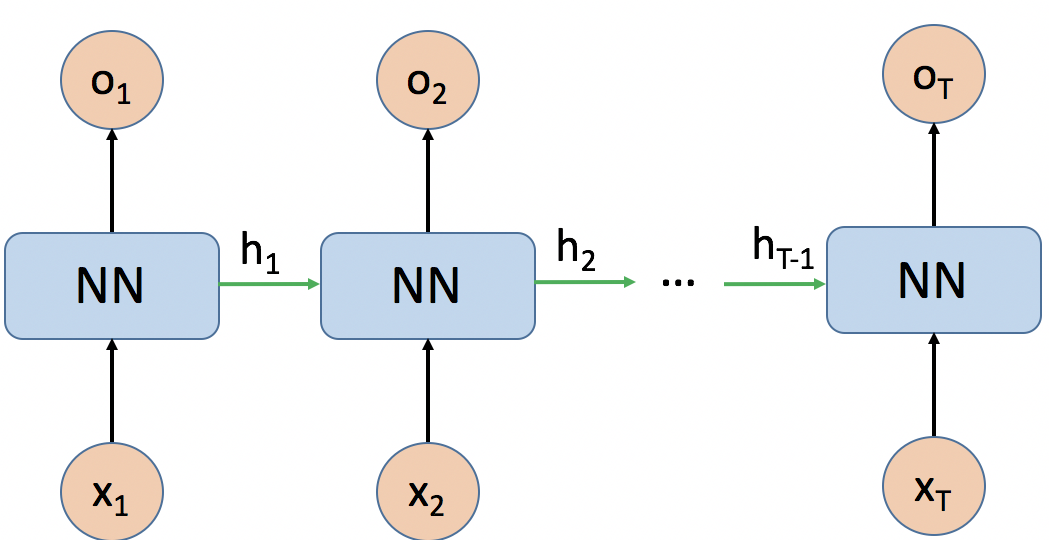
\includegraphics[scale=0.4]{images/ch3_RNN.png} 
\caption{遞迴式類神經網路}
\label{ch3_RNN}
\end{figure}
遞迴式類神經網路因其有記憶性,每個時間點的輸出,會依據之記憶跟現在時間點的輸入改變,如圖~\ref{ch3_RNN}所示。所以依照其特性,可以將語音文件一一給入模型中,在最後的時間點的輸出,可以當做模型已經看過整個語音文件,產生的語音特徵向量。此想法跟序列對序列模型(Sequence-to-Sequence
Model)~\cite{sutskever2014sequence} 的編碼器(encoder)的概念相同,在機器翻譯(Machine
Translation)和自動摘要(Summarization)裡是很常見的模型。在機器翻譯中,會先將欲翻譯的文字先經編碼器(遞迴式類神經網路)編碼成向量。在自動摘要中,也會將整篇文章先經過編碼器變成向量。


\chapter{專注式類神經網路之口述詞彙偵測}
  \section{簡介}
在第\ref{ch3}章中,嘗試了直接將語音文件跟語音查詢詞編碼成向量,進行口述詞彙偵測。雖然表現不如非監督式的動態時間規劃,但至少實作出可以捨棄語音辨識系統的口述詞彙偵測。第\ref{ch3}章中,直接將語音查詢詞變成一個向量是很合理的,因為語音查詢詞只包含完整的查詢詞,並無多餘的部分,但語音文件為一整個段落,包含了許多並非查詢詞的資訊,導致產生出來的語音文件向量喪失了查詢詞的特徵。即使後面分類器在複雜,但因語音文件向量中喪失了查詢詞特徵,所以無法準確的分辨出來。本章將專注式機制引入,專注式機制可以使模型專注在某個地方,將多餘的資訊濾除。藉由專注式機制使模型能夠關注在查詢詞的部分,可以有效保留著查詢詞特徵在產生出來的語音文件向量中,則不會分心在其他非查詢詞的部分。所以本章藉由專注式機制產生出較好的語音文件向量,可以保留著查詢詞的部分,不會被其他多餘的詞彙影響,以提升口述詞彙偵測的效能。
\section{專注式機制}
專注式機制,在近年漸漸受到大家重視,專注式機制最早被應用於機器翻譯的領域上,該系統為先前\ref{seq2seq}章提到的編碼器-解碼器遞迴神經網路,能提供端對端機器翻譯。而該系統的特點為能夠根據前一個時刻的輸出,去側重當今時刻的資料中重要的部分;如此這種根據狀況進行「挑選」的技能是先前的其他類神經網路所無法比擬的。
現已出現一些模擬專注力的神經網絡架構,如記憶網絡(Memory
Network)~\cite{sukhbaatar2015end}、類神經圖靈機(Neural Turing
Machine)~\cite{graves2014neural}、 動態記憶網路(Dynamic
Memory
Network)~\cite{kumar2015ask}等等,這類模型統稱專注式模型(Attention-based
Model)。

專注式模型常應用在問答(Question
Answering,QA)系統上,讓機器可以針對提出的問題,回答正確的答案。當使用者輸入問題時,專注式模型可以幫助機器從資料庫中選擇相關資料,而將專注力放在相關的資料上,避免其他無關資訊干擾,藉此得到問題的答案。問答系統甚至已經從文字擴展到多媒體,機器可以依據圖片回答相關問題(如:圖中的人穿什麼顏色的衣服)~\cite{agrawal2015vqa},而專注式機制可以幫助模型將重心放在圖片中人的衣服上,來判斷衣服的顏色,不會受到圖片中其他物件影響。不只如此,專注式模型也被應用在自動新聞摘要~\cite{rush2015neural}、自動產生圖片/影像說明~\cite{xu2015show}、語音辨識~\cite{chan2016listen}~與機器自動翻譯等任務上~\cite{bahdanau2014neural}。

受到這些啟發,將專注式機制應用於口述詞彙偵測。在第\ref{ch3}章中,編碼器最主要的難處是當輸入序列相當長時,可能會有比較多雜訊在其中、或者許多部分是與整體資訊無關的,這些或多或少都會影響編碼出來的語音文件向量,進而影響分類器判斷結果的正確率。因此我們希望透過專注式機制的特性,建立在原本長短期記憶神經網路就能處理序列問題的基礎上,再自動從序列中挑出重要的部分並且忽略其餘跟查詢詞無關的部分,使其語音文件向量能夠包含著查詢詞的資訊,使平均準確率能夠提升。
\section{模型架構}
\subsection{系統架構簡介}
\begin{figure}[h]
\centering
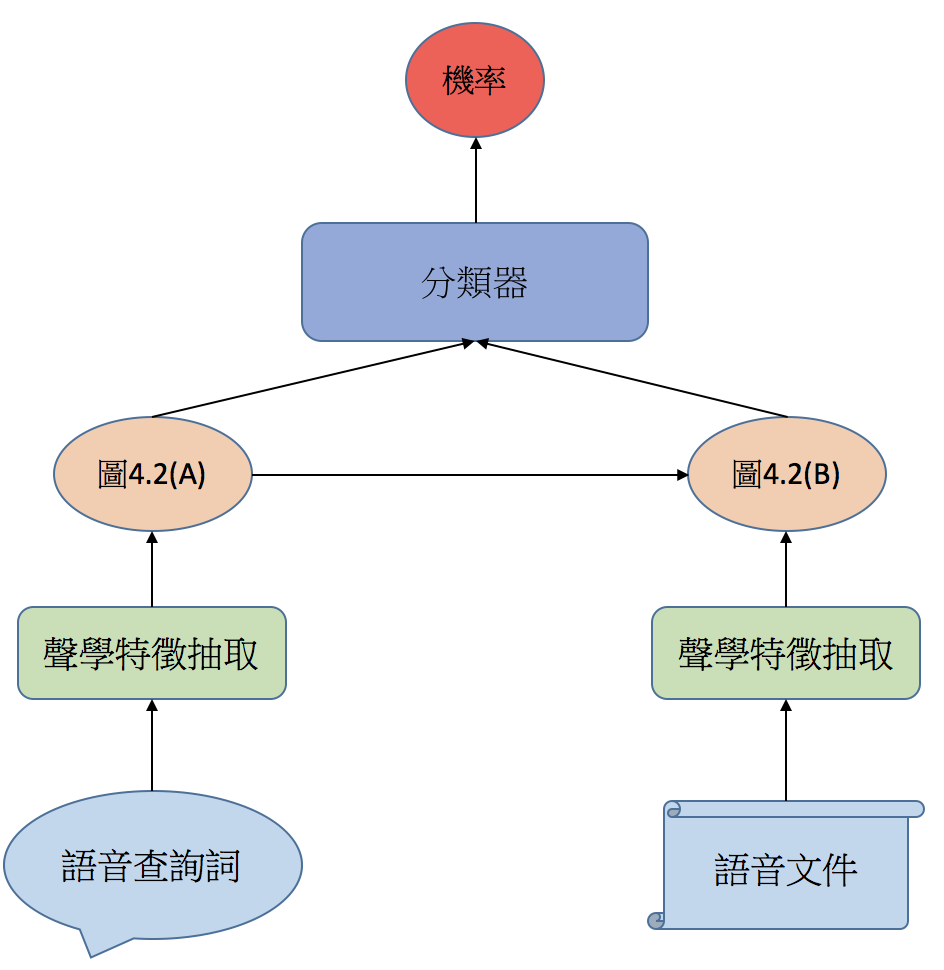
\includegraphics[scale=0.5]{images/ch4_model.png} 
\caption{模型架構圖}
\label{ch4_system}
\end{figure}
圖\ref{ch4_system}為本章節之系統架構圖。系統輸入部分包含了語音查詢詞跟語音文件,分別會經由聲學特徵抽取,轉變為39維的梅爾倒頻譜係數。首先,語音查詢詞的聲學特徵序列如同第\ref{ch3}章一樣被壓縮編碼並表示成為一向量,此向量稱之
$V_Q$ ,此部分會在\ref{ch4_query_vec}章在做介紹。產生出了 $V_Q$
,於\ref{ch4_doc_vec}章中將使用專注式機制找出跟語音查詢詞有關的部分,產生出較好的語音文件向量
$V_S$ 。最後,將 $V_Q$ 跟 $V_S$ 藉由分類器去預測查詢詞出現在文件中的機率,將在\ref{ch4_classify}章中作介紹。
\subsection{語音查詢詞之向量表示法}
\begin{figure}[h]
\centering
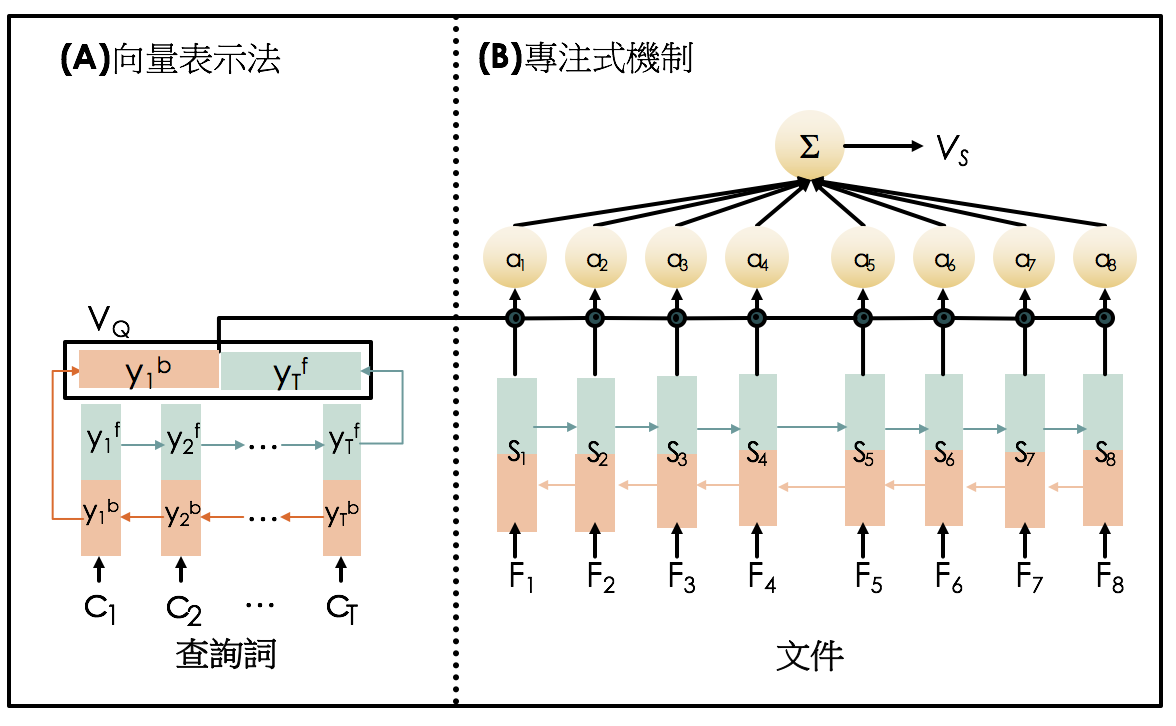
\includegraphics[scale=0.7]{images/ch4_att.png} 
\caption{專注式機制流程圖}
\label{ch4_att}
\end{figure}
\label{ch4_query_vec}
圖\ref{ch4_att}(A)為抽取 $V_Q$ 向量的介紹,將一連串的聲學特徵序列轉換為
$V_Q$ 的過程。輸入的查詢詞為
一長度T的序列,$C_1$, $C_2$,
...,$C_T$,其中 $C_i$ 均為39維梅爾倒頻譜係數。使用雙向式長短期記憶網路(Bidirectional
Long Short-term Memory
Network)作為編碼器的模型;其在輸入語音序列時,一個時間點只會讀取一個音框進去。在圖\ref{ch4_att}(A)中的第t個時間點時,正向(forward)長短期記憶網路的隱藏層輸出表示為
$y_t^f$ 、而反向(backward)長短期記憶網路之隱藏層輸出表示為 $y_{t}^b$
。在讀入所有的輸入序列之後,可在正向長短期記憶網路的最後一個時間點獲得一組隱藏層輸出向量
$y_{T}^f$ 、在反向長短期記憶網路的第一個時間點獲得 $y_{1}^b$
,並把他們串聯起來作為查詢詞的向量表示法 $V_Q$ , $V_Q
= [y_T^b || y_1^f]$ 。
\subsection{專注式機制與語音文件表示法}
在圖\ref{ch4_att}(A)中獲得查詢詞的向量表示法 $V_Q$
之後,之後將利用畫重點機制配合遞迴神經網路來對於語音文件的序列進行編碼,得到向量
$V_S$
,如圖\ref{ch4_att}(B)所示,語音文件的內容其實是一相當長的聲學特徵序列,但圖中我們簡化為八個音框,我們同樣使用雙向式長短期記憶網路來作為編碼的工具,其中在第t個時間點時,輸入詞彙的向量表示
$S_t$ 為正向長短期記憶網路與反向長短期記憶網路隱藏層輸出的串聯,$S_t
= [ y_t^f || y_t^b ]$。
接著我們引入專注式機制,來衡量查詢詞向量 $V_Q$
與語音文件內音框的關聯性高低,第 t 個時間點的語音文件向量 $S_t$
之專注式權重 $\alpha_t$ 為 $V_Q$ 與 $S_t$ 的相關程度,$\alpha_t=
S_t \odot
V_Q$,其中$\odot$表示兩向量之間的相關程度運算。相關程度的運算自己定義的,可以是簡單的歐式距離(Euclidean
Distance)、餘弦相似性(Cosine Similarity),也可使用類神經網路來計算,將兩向量丟入類神經網路去計算相關程度。
在本章中採用餘弦相似性當作相關程度,如式子\ref{cos_sim}所示:
\begin{equation}
	\label{cos_sim}
	\alpha_t = S_t \odot V_Q = \frac{S_t \cdot V_Q}{|S_t||V_Q|}
\end{equation}

接下來,對於所有的專注式權重 $\alpha_t$ 進行正規化,成為
$\hat{\alpha}_t$ ,正規化的方式有兩種。
\begin{itemize}
	\item{尖銳(Sharpening)正規化}
		
		我們將專注式權重透過軟式最大化(Softmax)之活化函數進行正規化:
		\begin{equation}
			\hat{\alpha}_t =
			\frac{exp(\alpha_t)}{\sum_{t=1}^{T} exp(\alpha_t)}
		\end{equation}
		由於可以確實降低資料的雜訊,此方式已被現存其餘專注式機制的相關研究所廣泛使用。
	\item{平滑(Smoothing)正規化}
		
		尖銳正規化偏好於注意一個點,因此一整個專注式權重集 $
		\boldsymbol{\alpha}
		= (\alpha_1,\alpha_2, ...,
		\alpha_T)$
		可能只會有某個向量 $\alpha_t$ 的權重特別高,其餘資訊皆被捨去。這樣的特性有可能降低口述詞彙偵測的表現。因此另外設計了一種正規化表示法,能夠考慮更多重要的點,此種方式也讓模型的多樣性因而增加。我們將原本算式中的指數函數改成S型函數(Sigmoid Function)$\sigma$:
		\begin{equation}
			\hat{\alpha}_t =
			\frac{\sigma(\alpha_t)}{\sum_{t=1}^{T}\sigma(\alpha_t)}
		\end{equation}

\end{itemize}

最後對於所有的語音文件向量 $S_t$
進行加權平均,使用的權重便為正規化後的專注式權重 $\hat{\alpha_t}$
,得到代表語音文件的向量 $V_S$,$V_S
= \sum_{t} \hat{\alpha_t} S_t$。
\label{ch4_doc_vec}
\subsection{分類器}
最後模型的輸出分數由分類器來決定的。分類器有很多種模型,常見的有支撐向量機(Support
Vector Machine)、類神經網路、貝氏分類器(Bayes
classifier)、決策樹(Decision
Tree)等等。在此章中,以多層類神經網路當作分類器,另外還使用語音文件向量 $V_S$
跟語音查詢詞向量 $V_Q$ 的餘弦相似度當作輸出分數為兩種產生分數的方式。
\label{ch4_classify}
\section{實驗與分析}
\section{本章總結}


%\chapter{非監督式學習語音向量之口語詞彙偵測}
%  \label{ch5}
\section{簡介}
在前一章節,利用專注式機制學習較好的向量表示,成功將平均準確率大幅提升,然而產生的查詢詞向量跟語音文件向量,就算為相似發音的詞,如hand跟hands,他們的向量表示卻大不相同。在本章中,想引入語音詞向量(Audio
Word2vec)的概念,能夠使模型學到詞的相關性,且語音詞向量是非監督式的學習方法,跟動態時間規劃的方法一樣,想嘗試以非監督式的方法,也能夠有進步。在語音詞向量模型中,會有每段詞的語音序列,才能夠訓練並產生出語音詞向量。但是我們在語音文件的部分,並無法得知每個詞的段落,所以本章想嘗試將即使不切出一段詞的語音序列而是將整段語音文件去產生出語音詞向量,並藉由分類器依據查詢詞的語音詞向量跟語音文件的語音詞向量判斷語音文件是否出現查詢詞。

\section{語音詞向量}
語音詞向量的概念為詞向量(Word Vector)的延伸,詞向量又稱詞嵌入(Word
Embedding)能夠將詞轉成有意義的向量。原本詞的表示方法常用的為是1-of-N編
碼(1-of-N
Encoding),也就是產生一個維度$N$的向量,$N$為辭典的詞數目,每一維度對應到一個詞,一個詞向量只有在該詞所對應到的維度其值為$1$,其$N-1$個維度的值都是$0$。此種表示法有其缺點,首先,$N$的維度都在數萬至數十萬的量級,導致詞向量的維度非常大。再者,此種表示法將所有的詞是為獨立,即便為兩個同義詞(Synonym),他們的1-of-N編碼之間也毫無關聯。而詞嵌入表示能夠產生分佈式表示(Distributed
Representation),將詞由原本的$N$維降低為幾百維度,且每一維度不在只有$1$或$0$,而是一連續的實數。且將語意關係或句法結構的關係,用兩個向量之間的歐式距離(Euclidean
Distance)或餘弦相似度(Cosine
Similarity)之大小就能呈現出來,例如母親與父親的歐式距離跟國王與皇后的歐式距離是相差不遠的。
語音詞向量則是希望在給定語音輸入下,也能夠產生固定維度的分佈式表示。
\begin{figure}[h]
\centering
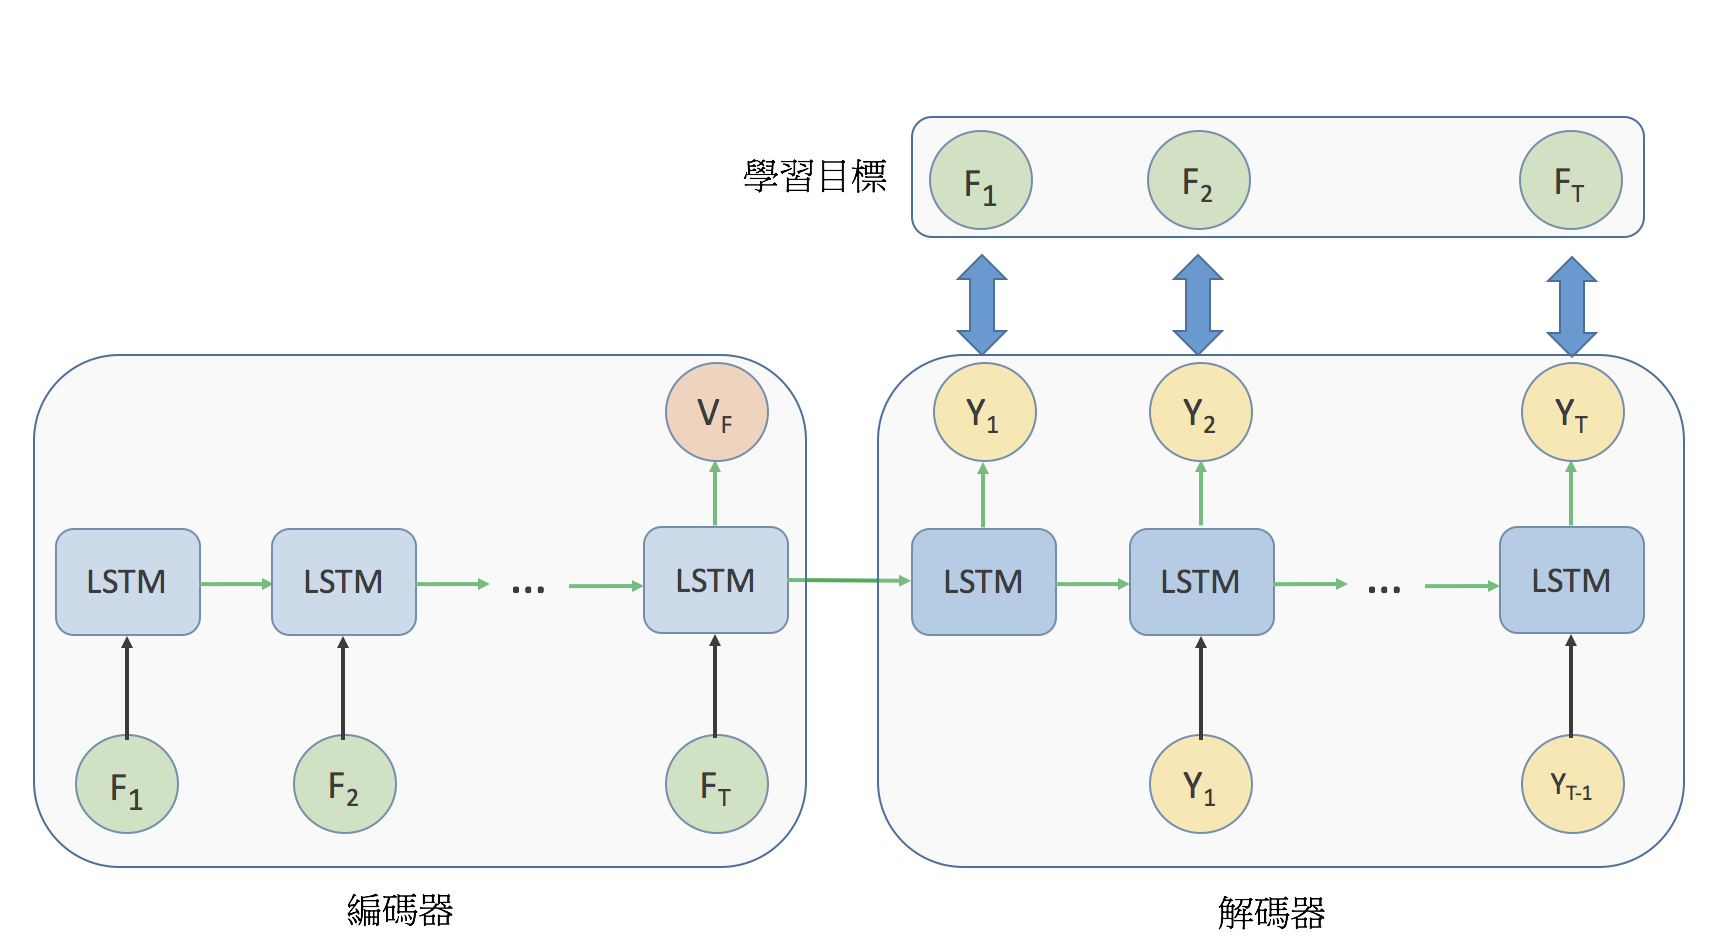
\includegraphics[scale=0.5]{images/ch5_seq2seq.png} 
\caption{語音詞向量模型圖}
\label{ch5_seq2seq}
\end{figure}
\label{ch5_seq2seq}

圖\ref{ch5_seq2seq}為語音詞向量的模型架構,基本概念仍為先前在\ref{seq2seq}章中提到的序列對序列的架構。編碼器會先將語音序列依據每個時間點$F_t$一一當作輸入,在看完整段序列後,產生一個維度固定的隱藏狀態。接著解碼器會將隱藏狀態當作初始狀態,一一產生出每個時間點的輸出$Y_t$。使其$Y_t$跟學習目標$F_t$要能夠完全相同,模型會嘗試降低$Y_t$跟$F_t$的方均根差(root-mean-square
error)。最後取其隱藏狀態當作語音序列的分佈式向量表示,即為語音詞向量。
\section{模型架構}
\subsection{模型簡介}
模型架構如圖\ref{ch5_seq2seq},編碼器將輸入的語音序列一一讀過產生出隱藏狀態,編碼器藉由隱藏狀態還原成原本的語音序列。唯一和語音詞向量不同的部分,訓練語音詞向量的資料為單個字語音序列,而此章的訓練資料並非單個字的語音序列,而是整個語音文件的序列。
\subsection{推理機制(Inference mechanism)}
在完成語音詞向量的訓練後,模型能夠藉由推理機制得到一個分數,利用此分數判別查詢詞出現在語音文件的機率。圖\ref{ch5_model}為本章推理機制示意圖,遞迴類神經網路編碼器會將查詢詞序列$Q_1,Q_2,...Q_T$編碼產生$V_Q$,語音文件序列$D_1,D_2,...,D_N$編碼產生$V_D$。接著,遞迴類神經網路解碼器會將$V_Q$跟$V_D$還原成原本的語音序列$\hat{Q_1},\hat{Q_2},...\hat{Q_T}$、$\hat{D_1},\hat{D_2},...,\hat{D_N}$,希望使其跟原本的序列越相近。最後,依照查詢詞向量$V_Q$跟語音文件向量$V_D$的歐式距離的分數排序,計算出平均準確率。

圖\ref{ch5_model}上有分別畫出語音文件跟查詢詞的編碼器,但是編碼器為同一組的遞迴類神經網路,負責將語音文件跟查詢詞編碼成向量。
\begin{figure}
\centering
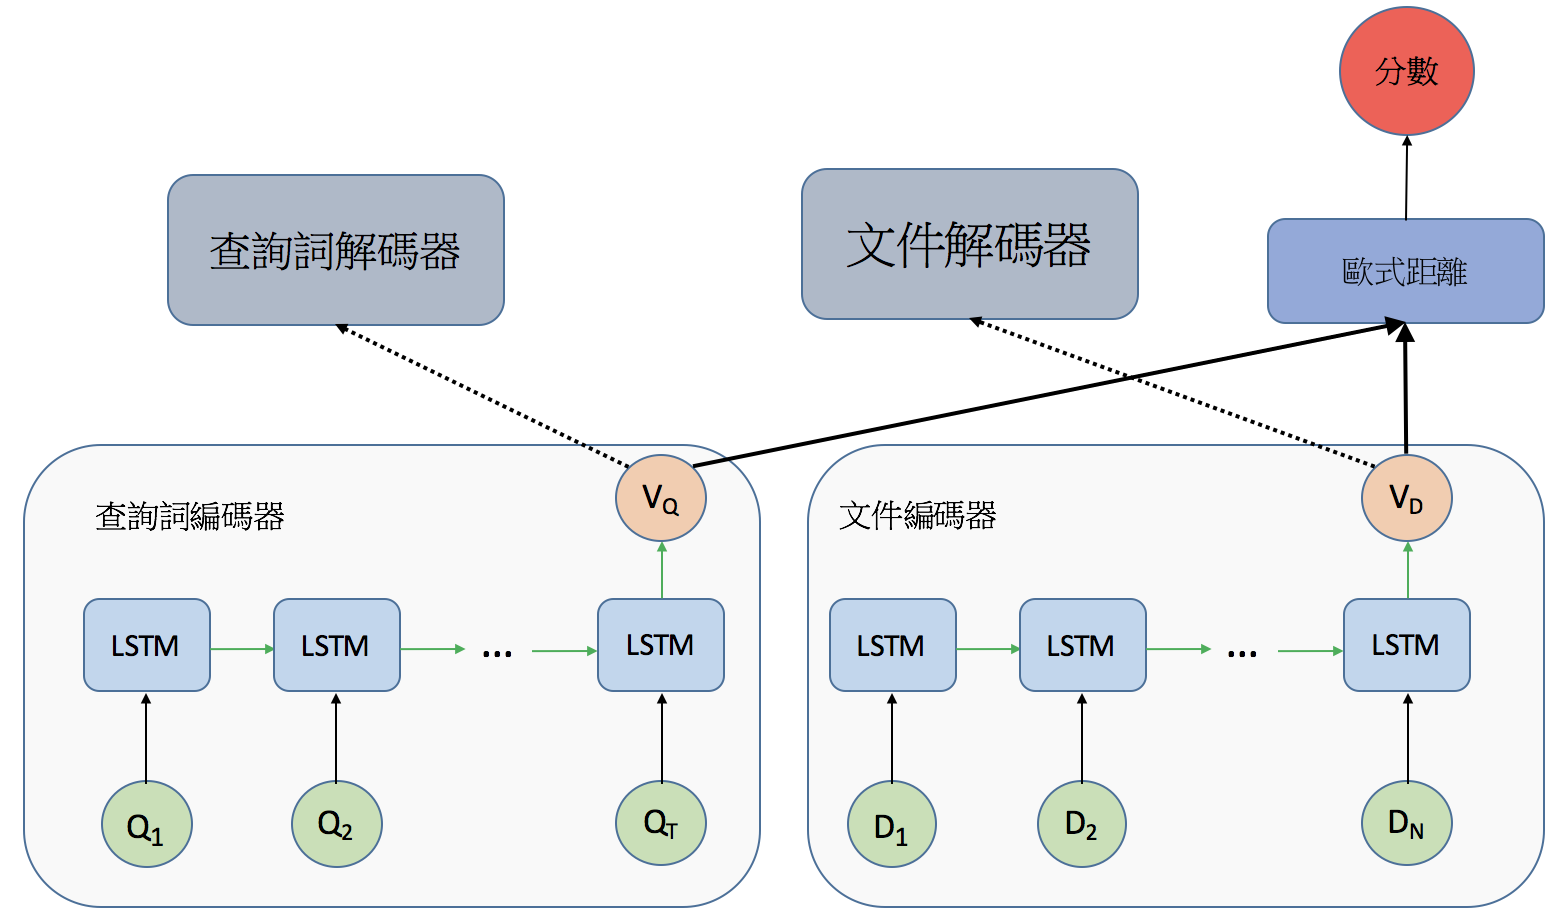
\includegraphics[scale=0.5]{images/ch5_model.png} 
\caption{模型推論機制示意圖}
\label{ch5_model}
\end{figure}
\subsection{訓練方式}
此時因模型需要能夠還原成原本的語音序列,其損失函數為均方根差如式\ref{eq:ch5_RMSE},使其編碼向量經過解碼器後的輸出跟其原始語音序列越相近。
\begin{equation}
\label{eq:ch5_RMSE}
L_{rmse} (\bold{x},\bold{y}) = \sum_{i=1}^{T}
RMSE(\bold{x}_i-\bold{y}_i) = \sum_{i=1}^{T} \sum_{j=1}^D \sqrt{(x_{ij}-y_{ij})^2}
\end{equation}
其中RMSE為方均根差,$\bold{x}$為輸入之語音序列,$\bold{y}$為模型還原之語音序列,$\bold{x}_i$為時間點$i$之聲學特徵,$\bold{y}_i$
為時間點$i$之模型還原聲學特徵,T為輸入序列長度,D為聲學特徵向量維度。最佳化演算法採用Adam演算法,採用二次正規化並給予權重0.001。

\section{實驗與分析}
\subsection{實驗設定與基準實驗}
\begin{itemize}
\item{實驗設定}

訓練語料為LIBRISPEECH 的英語語料,從train-clean-360
取出500種查詢詞,30,000個語音文件當作訓練語料。測試語料跟章節\ref{ch4}的設定相同,分成測試集$1$(查詢詞聲學特徵跟訓練語料相同)、測試集$2$(查詢詞聲學特徵跟訓練集不同)、測試集$3$(查詢詞未出現在訓練集)。
\item{基準實驗}

基準實驗仍為利用動態時間規劃得到的分數,在分別在測試集$1$得到0.6173的平均準確率,測試集$2$得到0.5778的平均準確率,測試集$3$得到0.5668的平均準確率。
\end{itemize}
\subsection{實驗結果與分析}
表\ref{table:ch5_a2v}為實驗之結果,在此章比較了不同層數的長短期記憶網路,而每層的記憶網路細胞個數為$128$個。從表中可以看出,利用語音詞向量的結果跟基準實驗差異不大,只有在層數較深的模型下,才略贏基準實驗。

動態時間規劃跟語音詞向量皆為非監督式的學習方法,所以都不需要利用到標記的資料,然而語音詞向量仍須有訓練語料才能夠學習,這是語音詞向量的劣勢。且本章並未將語音文件切成文字片段在進行訓練,而是以整段語音文件進行訓練,這表示產生出來的向量代表了整個語音文件,並不是表示單一個詞,而計算語音查詢詞跟語音文件之間的歐式距離,若語音文件出現跟查詢詞相似的詞但未出現查詢詞,此時利用歐式距離判別會產生出偏差,為此方法的一大缺失。但語音詞向量在此表現卻能跟基準實驗抗衡,是蠻意外的。

\begin{table}[ht]
	 \centering
	 \caption{語音詞向量之實驗結果}
	 \label{table:ch5_a2v}
	 \begin{tabular}{|c|c|c|c|}
		 \hline
		 模型架構 & 測試集1 & 測試集2 & 測試集3 \\
		 \hline
		 基準實驗 & 0.6173 & 0.5778 & 0.5678\\
		 \hline
		 一層長短期記憶網路& 0.6040 & 0.5890 & 0.5793 \\
		 \hline
		 兩層長短期記憶網路& 0.6160 &0.6038 &0.5988\\
		 \hline
		 三層長短期記憶網路& {\color{red}0.6223} &0.6127 &0.6011\\
		 \hline
	   \end{tabular}
\end{table}


\begin{figure}
\centering
\subfloat[]{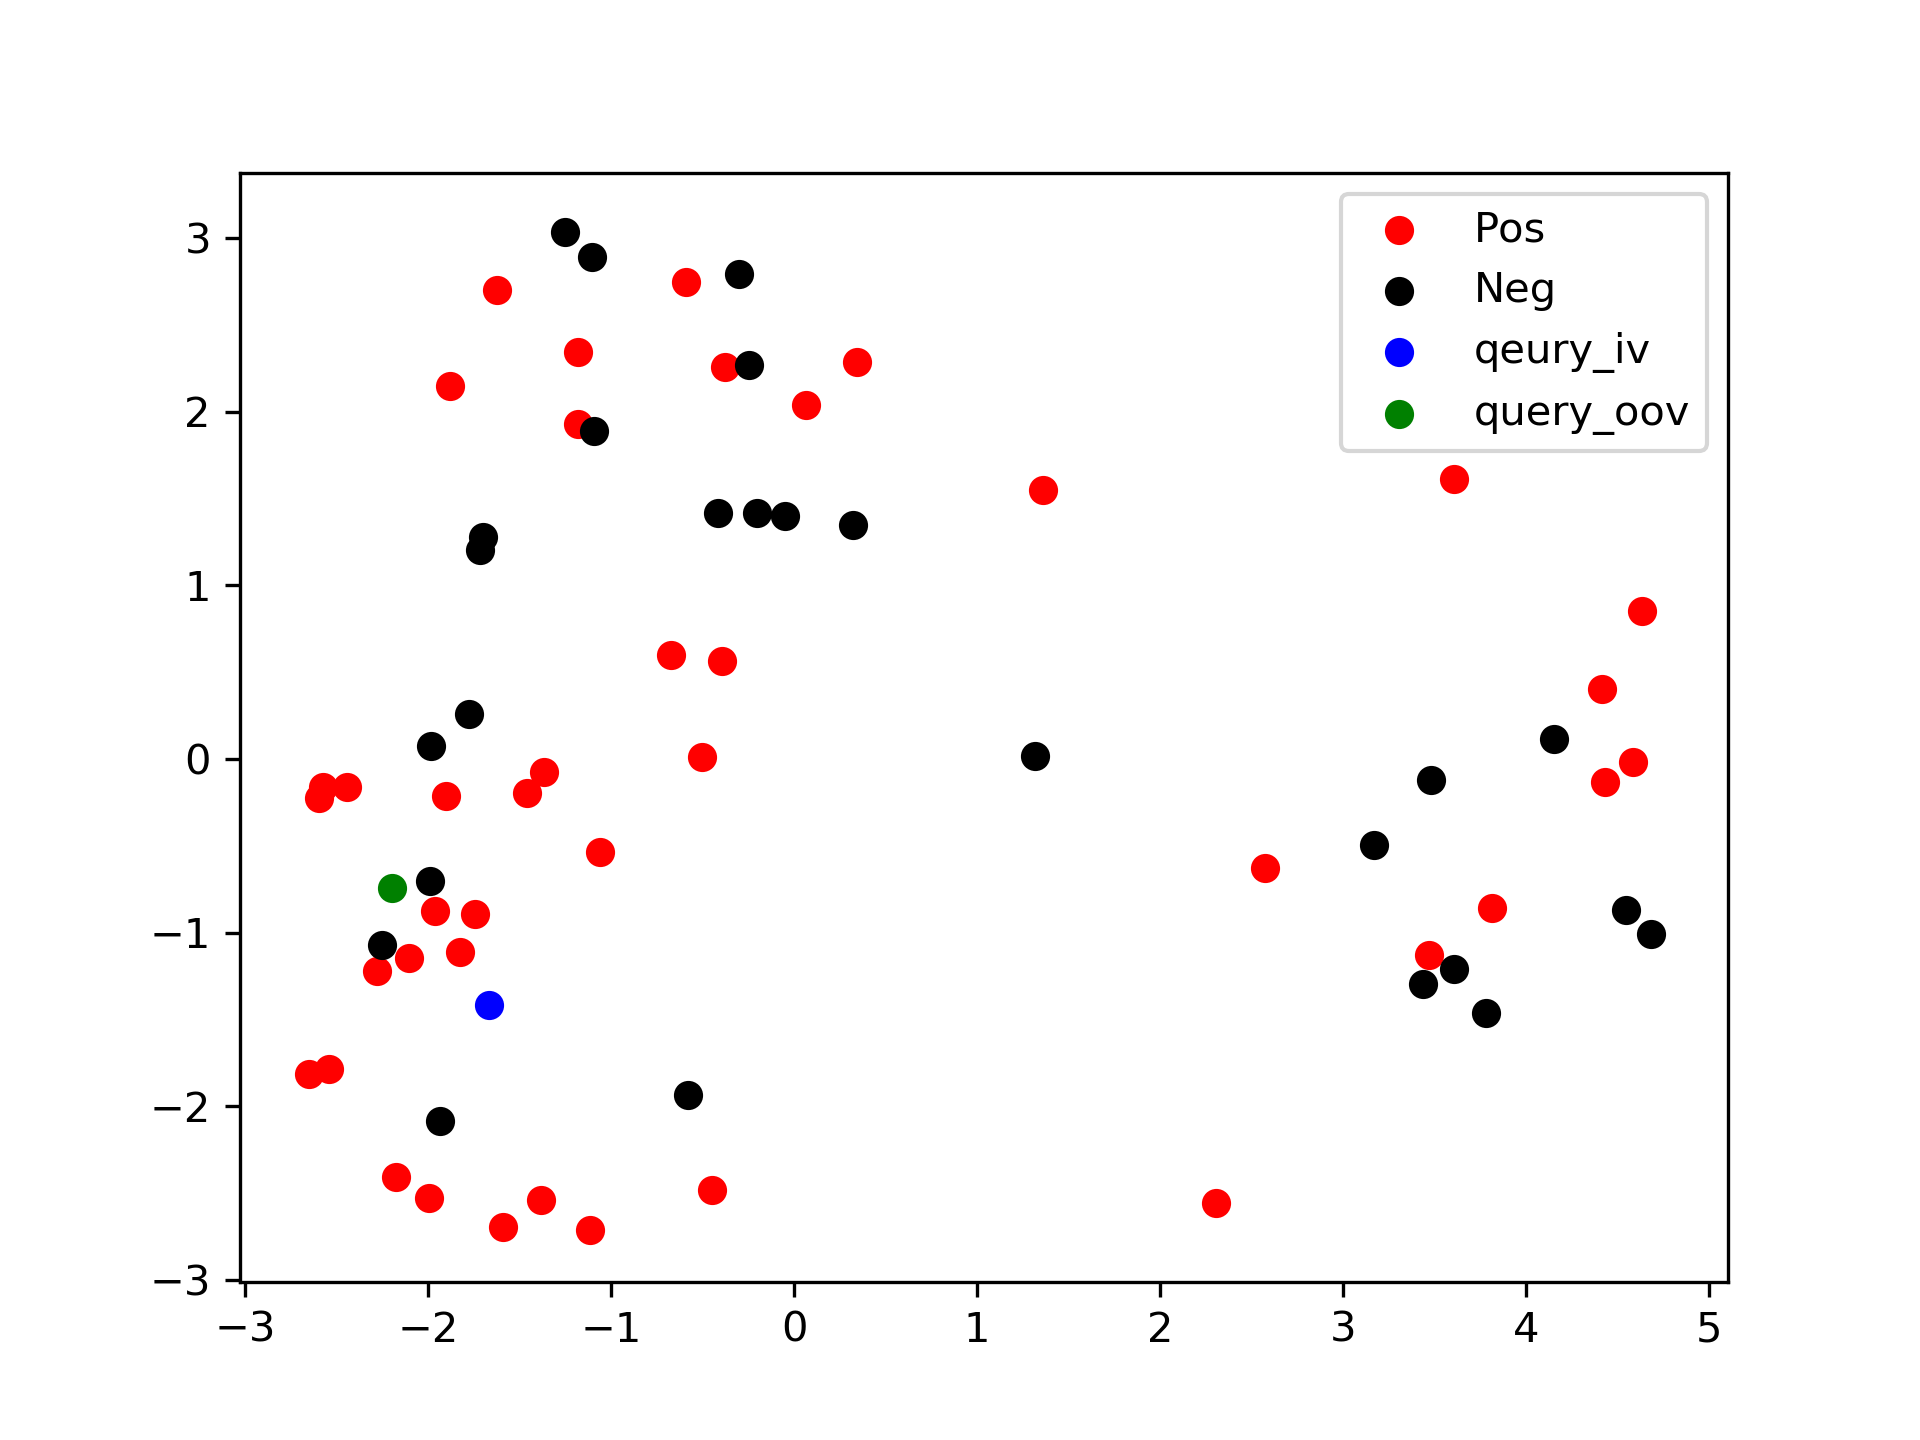
\includegraphics[scale=0.7]{images/ch5_pca1.png}}
\\
\subfloat[]{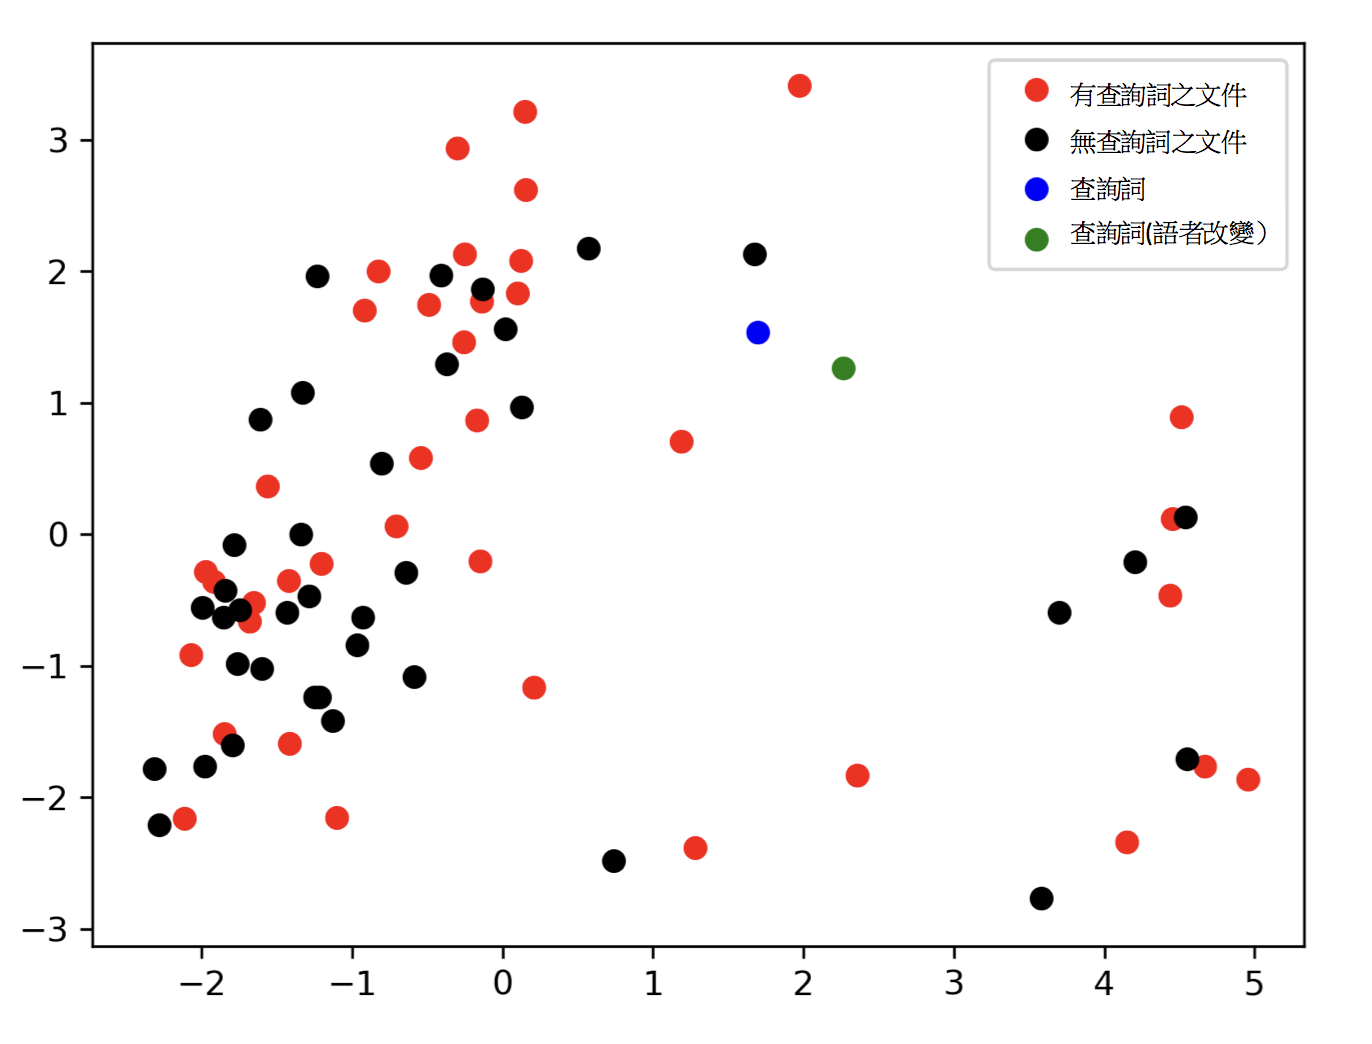
\includegraphics[scale=0.7]{images/ch5_pca2.png}}
\\
\caption{語音詞向量視覺圖}
\label{fig:ch5_vis}
\end{figure}


圖\ref{fig:ch5_vis} 為將查詢詞跟文件的語音詞向量,藉由主成份分析(Principal
Components
Analysis)\cite{dunteman1989principal}將高維的語音詞向量降成兩維,所畫出的圖。圖上紅點代表查詢詞出現的文件(Postive),黑點代表未出現查詢詞之文件(Negative),藍點為出現在訓練集的查詢詞聲學訊號,綠點為未出現在訓練集的查詢詞聲音訊號。
可以從圖上明顯地看出,依文件跟查詢詞的歐式距離作為判定不太可行的,語音文件的向量包含的是整個文件的資訊,跟查詢詞的向量是有極大差異的。但可以看出兩張圖中,不同聲學特徵的查詢詞兩者的歐式距離是近的,代表語音詞向量仍有學習到相同查詢詞的特性。圖\ref{ch5_query_vis}將查詢詞的語音詞向量透過主成份分析畫成的二維圖,可以看出DRIPPING跟JOINING為一群,PRECAUTION跟AVERSION也很相近。雖然查詢詞的訓練資料很少,但語音詞向量仍有抓到其查詢詞的特性。

\begin{figure}[h]
\centering
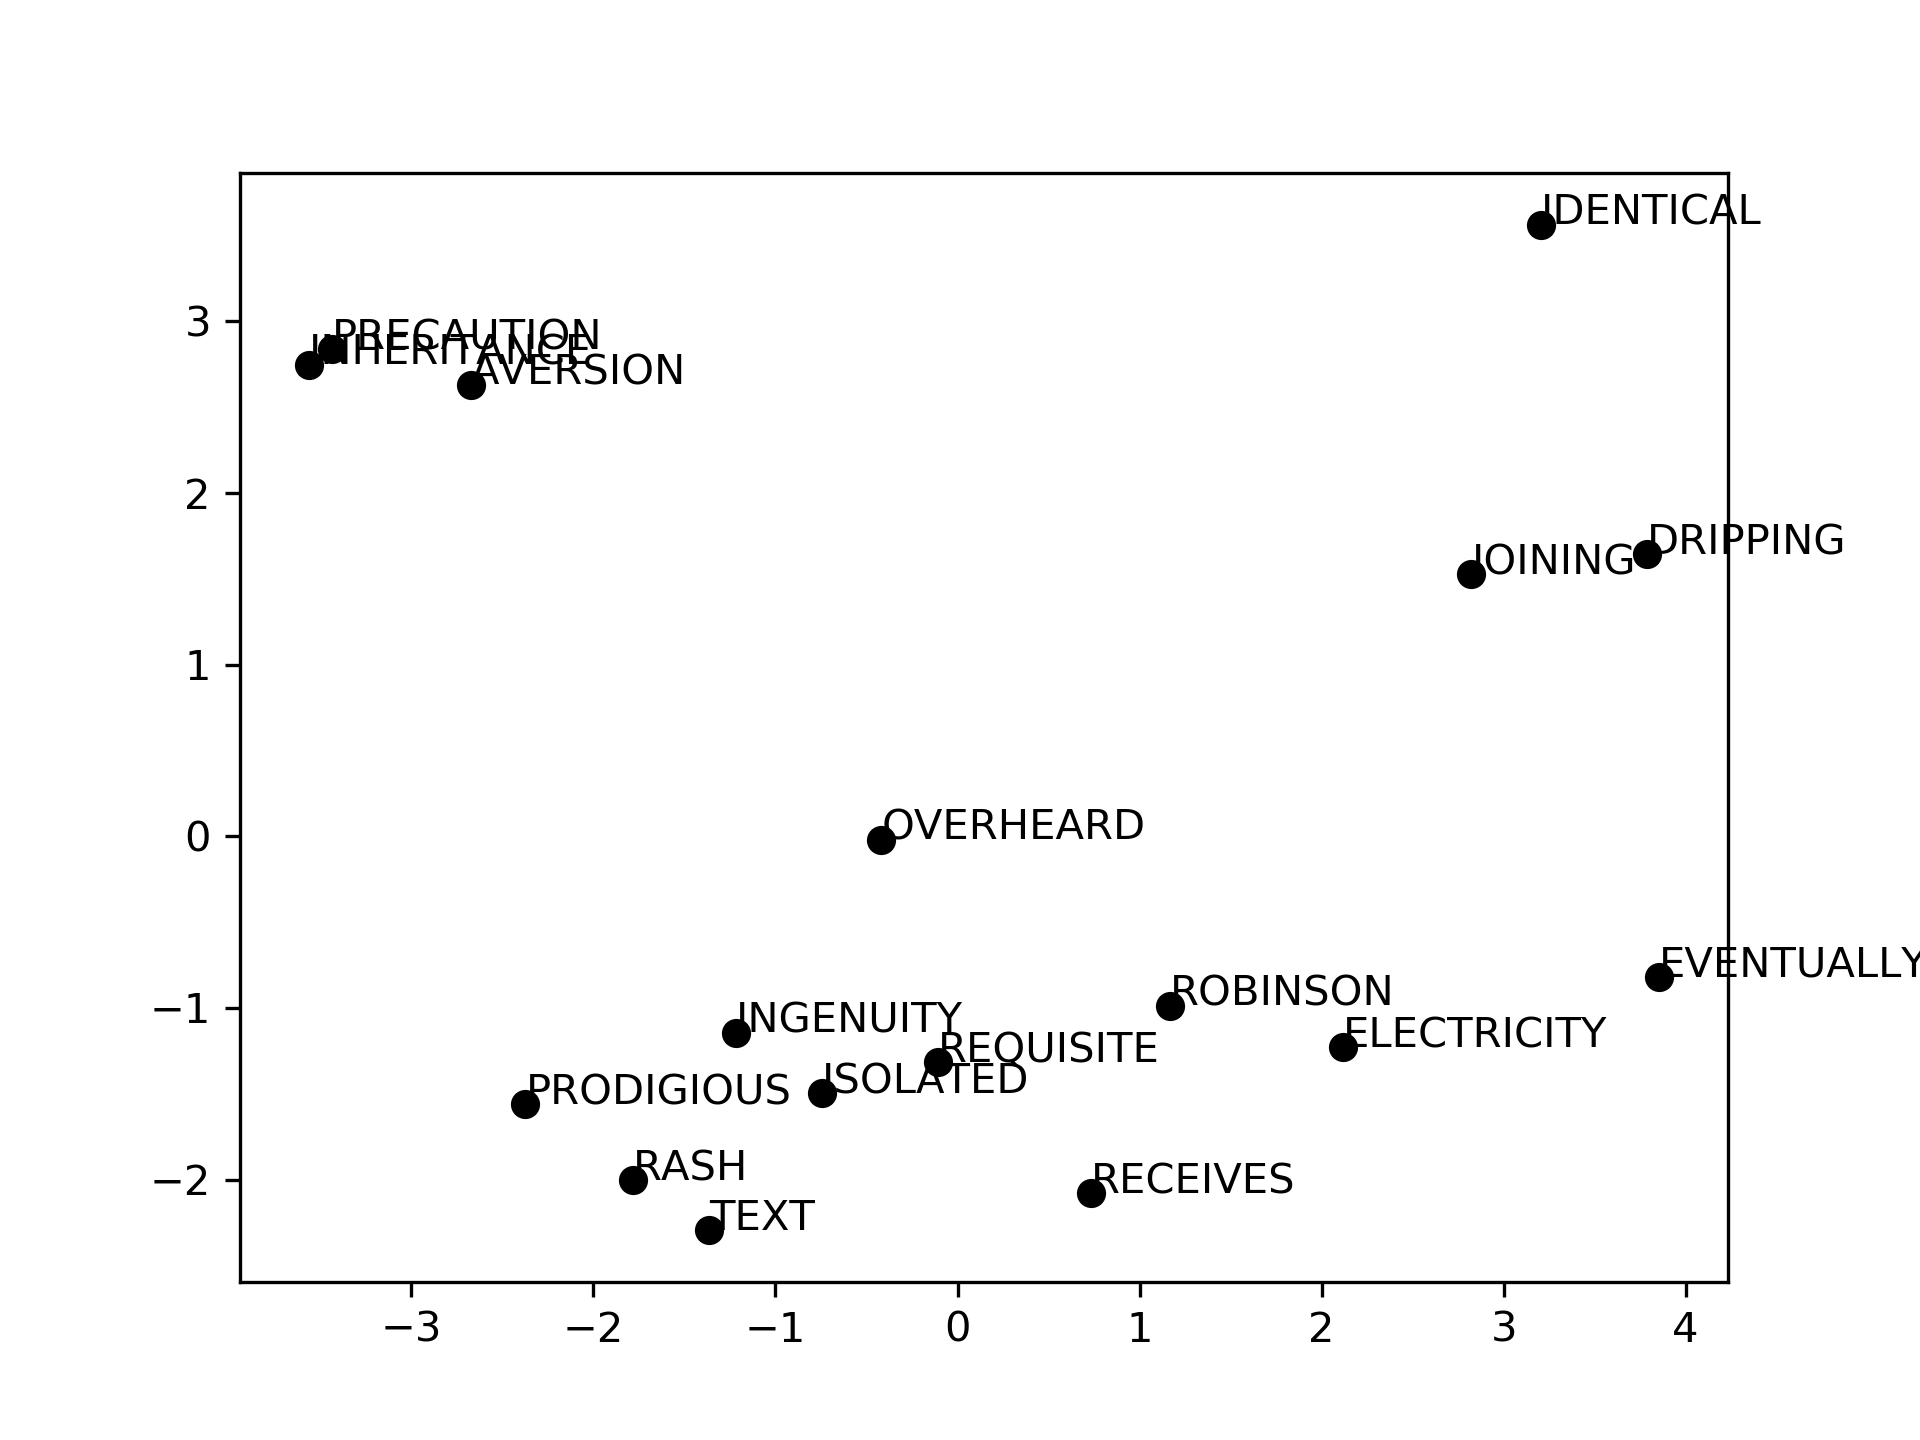
\includegraphics[scale=0.7]{images/ch5_query_vis.png} 
\caption{查詢詞之語音詞向量視覺圖}
\label{ch5_query_vis}
\end{figure}
\section{本章總結}
此章中利用了語音詞向量的概念,將未切段的語音文件直接進行訓練語音詞向量的模型。將語音文件與語音查詢詞分別產生其語音詞向量,利用它們之歐式距離來判定是否出現查詢詞。語音詞向量為非監督式學習,跟基準實驗動態時間規劃相同,也能夠產生與基準實驗相抗衡的表現。將語音詞向量視覺化後,證明利用整段文件去訓練語音詞向量,產生出來的向量跟查詢詞的歐式距離並無相關性。

%\chapter{在Google Glass上實作個人化的語音翻譯與新聞檢索系統}
%  \label{ch6}
\section{簡介}
由於第\ref{ch4}章,專注式機制對於系統表現有蠻大的幫助。且第\ref{ch5}章中,非監督式學習的語音詞向量,也有小幅的贏過動態時間規劃,若能夠將部分有標注的資料去微調模型,說不定能有更大的進步。所以在此章中,想將第\ref{ch5}章的語音詞向量跟第\ref{ch4}的專注式機制合併,變成半監督式學習法(Semi-Supervised),使用部分標記資料跟部分非標記資料來訓練,希望進而相輔相成,使其效能能夠更進步。
\section{模型架構}
\subsection{模型簡介}
圖\ref{ch6_model}為本章的模型架構圖,其概念是將第\ref{ch4}章跟第\ref{ch5}章的模型做結合,首先語音查詢詞跟語音文件先分別抽出聲學特徵後,經過圖\ref{ch6_att}將一連串聲學特徵轉變為代表查詢詞之向量$V_Q$跟代表語音文件之向量$V_D$,之後經過類神經網路分類器,產生出查詢詞出現在語音文件的機率。同時,模型能夠藉由圖\ref{ch6_a2v},將產生之向量經由解碼器還原成原本聲學序列。

%圖\ref{ch6_model}為本章的模型架構圖,跟第\ref{ch4}章提出的模型相同。同樣地,語音文件跟語音查詢詞都會先從音訊檔案中抽取聲學特徵。接著遞迴類神經網路編碼器將語音查詢詞之聲學特徵轉變成語音查詢詞向量 $ V_Q$,如圖\ref{ch6_att}(A),而語音文件向量則是採用專注式機制,利用語音查詢詞向量$V_Q$跟每個時間點的語音文件去計算餘弦相似度當作專注式權重,最後依照權重得到語音文件向量$V_D$,如圖\ref{ch6_att}(B)所示。得到$V_Q$跟$V_D$後,丟入分類器產生查詢詞出現在文件的機率。
\begin{figure}
\centering
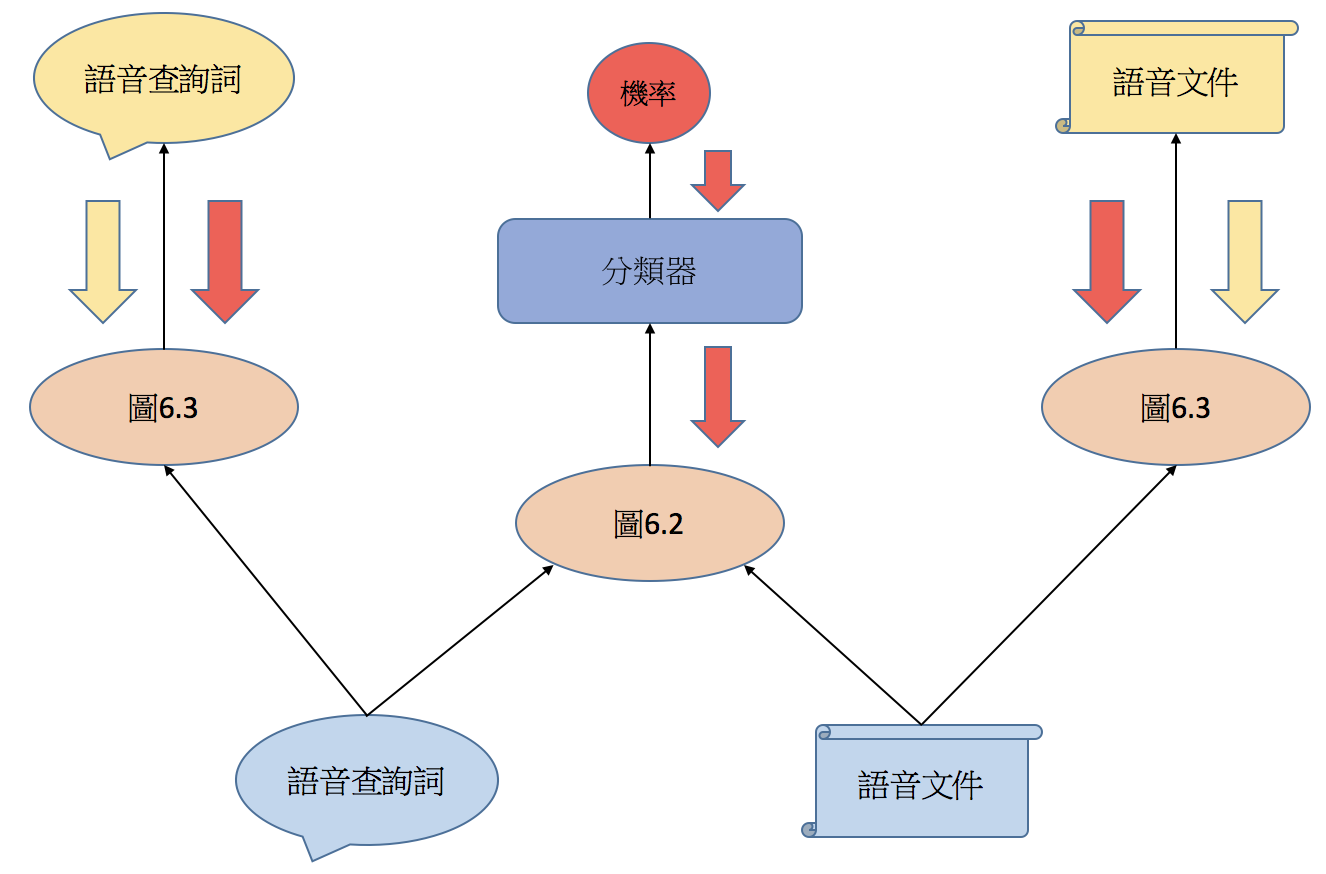
\includegraphics[scale=0.5]{images/ch6_model.png} 
\caption{模型架構圖}
\label{ch6_model}
\end{figure}
圖\ref{ch6_att}為產生查詢詞向量$V_Q$跟語音文件向量$V_D$的方法,第\ref{ch4}章的方法一模一樣,語音查詢詞經過遞迴類神經網路後,取其最後一個時間點當作$V_Q$,藉由$V_Q$與每個時間點遞迴類神經網路的語音文件向量輸出計算餘弦相似度,獲得一長度跟語音文件相同的權重值後,進行加權平均,來得語音文件向量$V_D$。

\begin{figure}
\centering
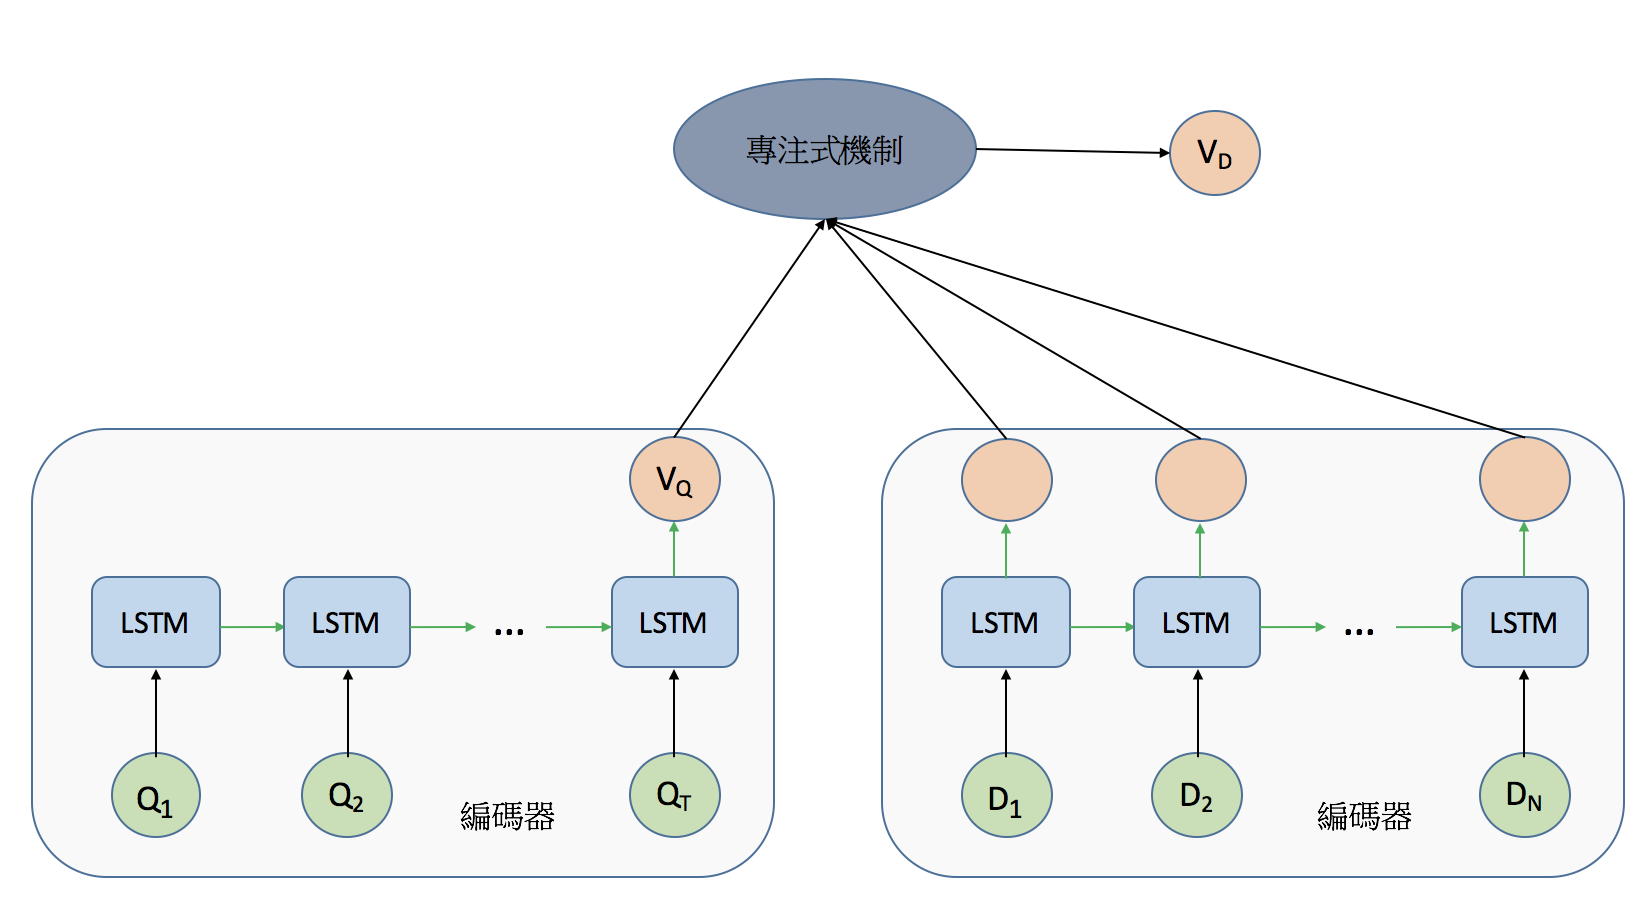
\includegraphics[scale=0.5]{images/ch6_att.png} 
\caption{專注式機制圖}
\label{ch6_att}
\end{figure}
圖\ref{ch6_a2v}為跟第\ref{ch5}章相同的序列對序列模型,將聲學序列經過遞迴類神經網路後產生的隱藏狀態,藉由解碼器轉回原本之聲學序列。此模型在此可以看做一正規化的機制,限制編碼器產生的向量不僅能精準的分類出查詢詞是否出現在語音文件,同時最後的隱藏狀態應該能夠保留著整段聲學序列的資訊。如此模型就不能單純做好分類問題,而必須同時達到其他目標,進而避免模型發生過度貼合之情形。
\begin{figure}
\centering
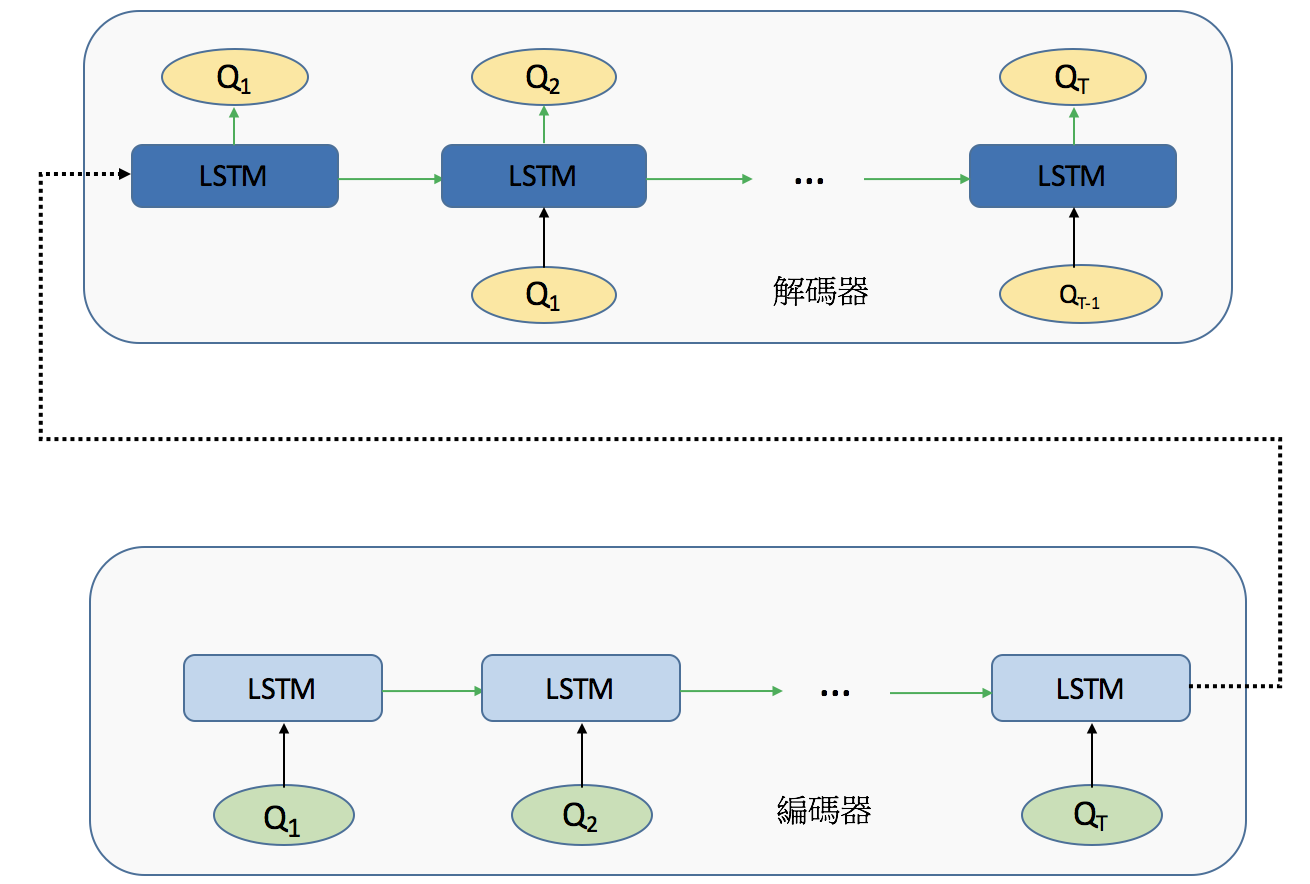
\includegraphics[scale=0.5]{images/ch6_a2v.png} 
\caption{語音詞向量正規化機制圖}
\label{ch6_a2v}
\end{figure}
\subsection{訓練方式}
此時因模型為多任務學習(Multi-Task
Learning),模型需要同時分類正確,且能夠還原成原本的語音序列。其損失函數會對於其任務有所不同,其一為交叉熵如式\ref{eq:ch5_LCE},為了提高口述詞彙偵測的正確率。
\begin{equation}
\label{eq:ch5_LCE}
L_{CE}(\bold{x} , \bold{y} , \theta) =KL(\bold{y} || f_{\theta}(\bold{x}))= KL( \bold{y} ||\hat{\bold {y}} )  = - \log \hat{y}_{l} 
\end{equation}
其中KL為克雷散度,$\bold{y}$為正確答案,$\hat{\bold{y}}$為模型預測之結果,$\hat{y_l}$為模型給正確標籤的分數。
而另一個損失函數為均方根差\ref{eq:ch5_RMSE},使其編碼向量能夠能夠完整還原最初之語音序列。
\begin{equation}
\label{eq:ch5_RMSE}
L_{rmse} (\bold{x},\bold{y}) = \sum_{i=1}^{T}
RMSE(\bold{x}_i-\bold{y}_i) = \sum_{i=1}^{T} \sum_{j=1}^D \sqrt{(x_{ij}-y_{ij})^2}
\end{equation}
其中RMSE為方均根差,$\bold{x}$為輸入之語音序列,$\bold{y}$為模型還原之語音序列,$\bold{x}_i$為時間點$i$之聲學特徵,$\bold{y}_i$
為時間點$i$之模型還原聲學特徵,T為輸入序列長度,D為聲學特徵向量維度。
\section{實驗與分析}
\subsection{實驗設定與基準實驗}
\begin{itemize}
\item{實驗設定}

	訓練語料為LIBRISPEECH 的英語語料,從train-clean-360
	取出30,000個語音文件當作訓練語料,用來訓練語音詞向量;取出70,000筆查詢詞跟語音文件配對,查詢詞共500個,用來訓練分類器。測試語料跟章節\ref{ch4}的設定相同,分成測試集$1$(查詢詞聲學特徵跟訓練語料相同)、測試集$2$(查詢詞聲學特徵跟測試集不同)、測試集$3$(查詢詞未出現在訓練語料)。
	
	在訓練的時候,會先訓練語音詞向量的部分,為監督式學習的部分,如圖\ref{ch6_model}上黃色箭頭的部分。接著才會訓練分類器。而在訓練分類器的同時,也會同時希望能夠還原成初始的語音序列,如圖\ref{ch6_model}上紅色箭頭部分。

\vspace{10cm}
\item{基準實驗}

	基準實驗仍為利用動態時間規劃得到的分數,在分別在測試集$1$得到0.6173的平均準確率,測試集$2$得到0.5778的平均準確率,測試集$3$得到0.5668的平均準確率。
\end{itemize}
\subsection{實驗結果與分析}
表\ref{table:ch6_exp}為本章實驗結果,編碼器為各種層數的長短期記憶網路,每一層有128個神經元。分類器使用四層的類神經網路,其架構為128-64-32-2。可以發現有了標記的資料進行訓練,使模型表現比第\ref{ch5}章的模型跟基準實驗的表現進步許多,然而加上了語音詞向量當作正規化,使模型同時要分類正確並由向量還原初始的語音序列。兩種任務無法達成互補的效果,使其平均準確率較第\ref{ch4}章的模型低了一個層級,不論使用幾層的編碼器,效能仍不及單純的專注式模型。
\begin{table}[ht]
	 \centering
	 \caption{專注式遞迴類神經網路實驗結果}
	 \label{table:ch6_exp}
	 \begin{tabular}{|c|c|c|c|c|}
		 \hline
		 \multicolumn{2}{|c|}{模型架構} & 測試集1 & 測試集2 & 測試集3 \\
		 \hline
		 \multicolumn{2}{|c|}{基準實驗} & 0.6173 & 0.5778 & 0.5678\\
		 \hline
		 \multicolumn{2}{|c|}{專注式模型} & 0.6523 & 0.6246 & 0.5754\\
		 \hline 
		 編碼器模型 & 分類器模型 & 測試集1 &測試集2 & 測試集3 \\
		 \hline
		 一層長短期記憶網路&\multirow{3}{*}{類神經網路} &
		   0.6232 &0.6005 & 0.5674\\
		 \cline{1-1}\cline{3-5}
		 兩層長短期記憶網路& & 0.6358 & 0.6035 & 0.5779 \\
		 \cline{1-1}\cline{3-5}
		 三層長短期記憶網路& & 0.6423 & 0.6104 & 0.5700 \\ 
		 \hline
	   \end{tabular}
\end{table}
\section{本章總結}
本章節將第\ref{ch4}章專注式機制跟第\ref{ch5}章語音詞向量的方法結合,使模型變為多任務學習,同時能夠將口述詞彙精準的找出,並藉由語音詞向量的訓練,使編碼器產生較好的向量表示,然而最後結果多任務學習拖累了原本主要的目的口述詞彙偵測的表現,並無達到相輔相成的效果。

%\chapter{結論與展望}
%  \section{結論}
本論文主要目的為不經過語音辨識系統達成口述詞彙偵測的目的。傳統的口述詞彙偵測系統的檢索效果好壞完全依靠著前面的語音辨識系統的辨識效果為何,若語音辨識系統錯誤率偏高,會嚴重影響檢索系統。且語音訊號經過了辨識系統,許多語音中珍貴的資訊如韻律、語速和語者特徵等就消失了。藉由類神經網路直接由語音訊號進行搜索,希望能夠避免掉語音辨識系統的影響。

第\ref{ch3}章中,提出了一個基本的模型架構,利用遞迴類神經網路將查詢詞聲學序列跟語音文件序列編碼成為一向量,藉由類神經網路判別查詢詞是否出現在語音文件中,雖然平均準確率輸給了動態時間規劃,但此模型已為捨棄掉語音辨識的檢索系統。

第\ref{ch4}章中,將第\ref{ch3}章的模型利用專注式機制改良,使其在編碼器產生語音文件的向量時藉由利用專注式機制,將多餘且跟查詢詞無關的資訊濾除,使其能夠專注在疑似查詢詞的位置。在此章中,將專注式權重視覺化後,發現在查詢詞位置的結束處,專注式權重都特別大,證明了模型有關注在查詢詞出現的位置,使其模型效能大幅提升。最後同時利用模型跟動態時間規劃,能夠使檢索效能再往上提升。

第\ref{ch5}章中,引入語音詞向量的概念,將整段語音文件去訓練語音詞向量,希望產生出的語音文件向量也能夠有語音詞向量的特性。而藉由查詢詞跟文件的語音詞向量的歐式距離,決定查詢詞是否出現在文件當中。將語音詞向量視覺化後,證明了文件跟查詢詞的歐式距離並無絕對的關係,且文件跟查詢詞的查詢詞有著不同的意義。在查詢詞中,能夠將發音類似的結尾分在同個區域。而在文件中,無法找出特別的分類關係。

在最後的第\ref{ch6}章中,將前幾章的模型做結合希望能夠有所進步,而實驗證明同時訓練語音詞向量並進行口述詞彙偵測,會使模型的效能變差一點,將語音詞向量當作正規化並無法幫助模型在口述詞彙偵測的表現。
\section{未來與展望}
首先,本篇論文其關鍵的部分在於專注式權重的計算,未來可以嘗試更多的專注式權重的算法,如由類神經網路產生出專注式權重或者將每個時間的編碼器產生的查詢詞向量跟語音文件向量都去產生一個專注式權重,進而改善模型的效能。

再者,本篇論文皆在討論查詢詞為語音的情況,未來也可以朝向查詢詞為人為輸入的文字,而直接由文字跟語音找尋其相似特徵,難度會比較高。因文字跟語音訊號本身有巨大的差異,要如何將語音和文字的配對是一個要思考的大問題。

最後,未來也可以朝向語意檢索的方向邁進,同樣不經過語音辨識,但能夠將查詢詞相關的文件也檢索出來。若能夠將語義的資訊放入編碼的向量中,則可利用查詢詞擴展,將查詢詞附近的向量也進行檢索,進而找出語意相關的文件。


%
% this file is encoded in utf-8
% v2.0 (Apr. 5, 2009)

%%% 參考文獻
\newpage
\phantomsection % for hyperref to register this
\addcontentsline{toc}{chapter}{\nameRef}
\renewcommand{\bibname}{\protect\makebox[5cm][s]{\nameRef}}
%  \makebox{} is fragile; need protect
\bibliographystyle{IEEEbib}  % 使用 IEEE Trans 期刊格式
\bibliography{thesis_bib}


%%% 附錄
%\input{my_appendix.tex}

%%% 自傳
%\newpage
%\chapter*{\protect\makebox[5cm][s]{\nameVita}} % \makebox{} is fragile; need protect
%\phantomsection % for hyperref to register this
%\addcontentsline{toc}{chapter}{\nameVita}
%\input{my_vita.tex}



\clearpage % to make sure all CJK characters are processed
\end{CJK}  %%% ZZZ %%%
\end{document} 
 
